\documentclass[10pt,a4paper]{article}
\usepackage[justification=centering]{caption}
\usepackage[pdfpagelabels,bookmarks,hyperindex,hyperfigures, hidelinks]{hyperref}
\usepackage[spanish]{babel}
\usepackage[utf8]{inputenc}
\usepackage[version=4]{mhchem}
\usepackage{alltt}
\usepackage{amsmath}
\usepackage{circuitikz}
\usepackage{epstopdf}
\usepackage{fancyhdr}
\usepackage{gensymb}
\usepackage{parskip}
\usepackage{lastpage}
\usepackage[version=4]{mhchem}
\usepackage{multirow}
\usepackage{pdfpages}
\usepackage{subcaption}
\usepackage{textcomp}
\usepackage{upgreek}
\usepackage{xfrac}
\usepackage{placeins}
\usetikzlibrary{arrows, decorations.markings}

% Print a DRAFT water mark on the document
% Comment to remove for final version
\usepackage{draftwatermark}
\SetWatermarkText{ DRAFT }
\SetWatermarkScale{5}

\setlength{\parskip}{0.6em}

% Set the indentation length 
\setlength{\parindent}{0em}

% Bibliography settings
\usepackage[backend=biber,style=ieee]{biblatex}
%\setbeamertemplate{bibliography item}{\insertbiblabel}
\addbibresource{major_paper.bib}

% Glossary entries
\usepackage[acronym, nomain]{glossaries}
\makenoidxglossaries

\newacronym{BMS}{BMS}{Battery Management System}
\newacronym{CAN}{CAN}{Controller Area Network}
\newacronym{UPS}{UPS}{Uninterruptible Power Supply}
\newacronym{VE}{VE}{vehículo eléctrico}
\newacronym{VVEE}{VVEE}{vehículos eléctricos}
\newacronym{IISB}{IISB}{Institute for Integrated Systems and Device Technology}
\newacronym{ARLB}{ARLB}{Aqueous rechargeable lithium batteries}
\newacronym{FPGA}{FPGA}{Field Programmable Gate Arrays}
\newacronym{EC}{EC}{Eficiencia Culombica}
\newacronym{TCR}{TCR}{Temperature Coefficient of Resistance}
\newacronym{DOD}{DOD}{Depth of Discharge}
\newacronym{OCV}{OCV}{Open Circuit Voltage}
\newacronym{SOC}{SoC}{State Of Charge}
\newacronym{MCU}{MCU}{Microcontroller Unit}
\newacronym{DB}{DB}{Diagrama de Bloques}
\newacronym{SOA}{SOA}{Secure Operation Area}
\newacronym{hri}{HRI}{human-robot interactions}
\newacronym{rnn}{RNN}{Recurrent Neural Network}
\newacronym{lstm}{LSTM}{Long Short-Term Memory}
\newacronym{Ion-Li}{Ion-Li}{Batería de Ion Litio}
\newacronym{Li-Po}{Li-Po}{Batería de Polímero de Litio}
\newacronym{CC}{CC}{Constant Current}
\newacronym{CV}{CV}{Constant Voltage}

\tikzstyle{vecArrow} = [thick, decoration={markings,mark=at position
	1 with {\arrow[semithick]{open triangle 60}}},
double distance=1.4pt, shorten >= 5.5pt,
preaction = {decorate},
postaction = {draw,line width=1.4pt, white,shorten >= 4.5pt}]
\tikzstyle{innerWhite} = [semithick, white,line width=1.4pt, shorten >= 4.5pt]
\graphicspath{{assets/}} 
\newcommand\reaction[1]{\begin{equation}\ce{#1}\end{equation}} 

\setcounter{MaxMatrixCols}{20}

\setlength{\headheight}{52pt}
\pagestyle{fancy}
\fancyheadoffset{0.5cm}
\fancyhead{}
\fancyhead[L]{
\includegraphics[scale=0.125]{FCEIA-logo.png}}
\fancyhead[C]{Universidad Nacional de Rosario\\
Facultad de Ciencias Exactas,Ingeniería y Agrimensura\\
Escuela de Ingeniería Electrónica}
\fancyhead[R]{
\includegraphics[scale=0.06]{LOGO-UNR-NEGRO.png}}

\renewcommand{\figurename}{Fig.}

\renewcommand\footrule{\begin{minipage}{0.95\textwidth}
    \hrule width \hsize   
\end{minipage}\par}

\setlength{\footskip}{30pt}
\fancyfoot[L]{\textit{Proyecto Final - F. Ceccarelli, M. Moya, L. Santos}}
\fancyfoot[C]{}
\fancyfoot[R]{\textit{Página \thepage{} de \pageref{LastPage}}}

\DeclareGraphicsExtensions{.bmp, .png, .jpg}

\renewcommand*\contentsname{Índice}

\topmargin = -1.5cm
\leftmargin = -1cm
\oddsidemargin = 0cm
\textheight = 24cm
\textwidth = 17cm


\begin{document}

\begin{titlepage}
    \begin{center}
	\begin{minipage}{.45\textwidth}
	    \flushleft
	    
\includegraphics[scale=0.25]{FCEIA-logo.png}
	\end{minipage}%
	\hspace{20mm}
	\begin{minipage}{.3\textwidth}
	    \flushleft
	    
\includegraphics[scale=0.1]{LOGO-UNR-NEGRO.png}
	\end{minipage}

	\vspace{15mm}

	\large{ \textbf{Universidad Nacional de Rosario}} \\[5mm]
	\textbf{Facultad de Ciencias Exactas, Ingeniería y Agrimensura} \\[5mm]
	Escuela de Ingeniería Electrónica \\[20mm]
	\Large {\textbf{Área de Gestión de Proyectos}}\\[1.5mm]
	\small {Ingeniería Electrónica} \\[20mm]
	\Large {\textbf{Proyecto Final}} \\[5mm]
	\Large{ \textbf{Estudio e Implementación de un Sistema de Administración de
	Baterías de Li-Ion de baja y mediana potencia}} \\[15mm]

    \end{center}

    \begin{minipage}[t]{0.6\textwidth}
	{\large\textbf{Autores:}}
	\begin{itemize}
	    \item [] Federico Ceccarelli (C-6241/3)
	    \item [] Martin Moya (M-6132/8)
	    \item [] Lucio Santos (S-4966/2)
	\end{itemize}
	\vspace{10pt}
	{\large\textbf{Directora:}}

	\begin{itemize}
	    \item [] Dra. Monica Romero
	\end{itemize}
	\vspace{10pt}
	{\large\textbf{Asesor:}}
	\begin{itemize}
	    \item [] Ing. Edgardo Arnejo
	\end{itemize}
    \end{minipage}

    \begin{minipage}[t]{0.35\textwidth}
	\flushleft
	\Large\textbf{Firma:}
    \end{minipage}

\end{titlepage}

\newpage

\begin{abstract}
    \noindent En el presente trabajo se detalla el proceso de desarrollo e
    investigacion de un administrador de baterias o, tambien conocido como,
    \acrshort{BMS} (del ingles \emph{\acrlong{BMS}}) compatible con un pack
    de baterias de iones de litio, capaz de estimar el estado de carga 
    utilizando filtros cuadraticos, balancear, proteger, cargar y 
    comunicar, a traves del protocolo \acrshort{CAN}, todas 
    las variables del mismo. El dispositivo es orientado a vehiculos 
    electricos de baja y mediana potencia, como por ejemplo, 
    bicicletas/monopatines hasta triciclos de transporte con carga
    y busca resolver mucha de las problematicas intrinsecas de 
    la tecnologia litio-ion, como por ejemplo, su volatilidad ante 
    operaciones fuera del area segura de operacion, 
    como tambien la falta de proyectos abiertos de esta indole en el mercado. 
    A pesar de estar caracterizado para vehiculos electricos, el mismo 
    puede ser aplicado a almacenadores de energia, tales como los paneles 
    solares, incluso hasta sistemas de alimentacion ininterrumpida, o \acrshort{UPS} 
    (del ingles, \emph{\acrlong{UPS}}).
\end{abstract}

\newpage
% Print table of contents
\tableofcontents

\newpage

\section{Introducción}

\noindent A partir de la relevancia que ha comenzado a tomar el 
calentamiento global en las últimas décadas y el inquietante impacto que 
el mismo tiene sobre la calidad de vida de las personas, se han intentado 
buscar distintas soluciones para apaciguar las principales causas que 
generan un deterioro del medio ambiente, entre ellas, se encuentra el 
desarrollo de nuevas fuentes de energía renovables y su aprovechamiento.

\noindent El \acrfull{VE} \emph{(fig. \ref{EV})} es considerado 
una de las transiciones tecnológicas más importantes de los últimos años 
debido a que no emiten dióxido de carbono ($\mathrm{CO_2}$) al medio 
ambiente y no utilizan combustibles fósiles para su funcionamiento, esto 
los convierte en uno de los avances tecnológicos más atractivos de los 
últimos tiempos teniendo en cuenta el avance del calentamiento global y el 
crecimiento del valor del petróleo.

\begin{figure}[h!]
    \begin{center}
	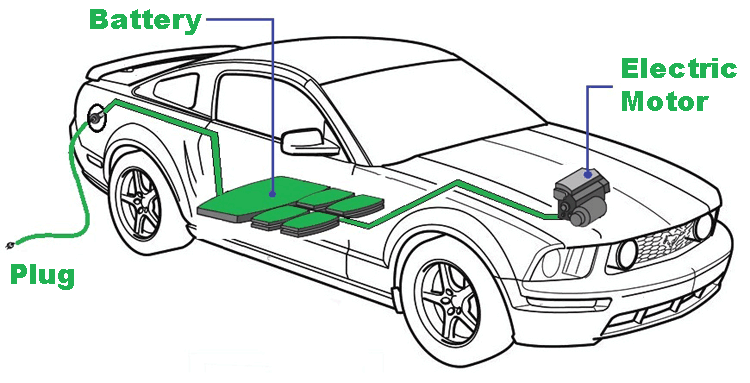
\includegraphics[width=0.7\textwidth]{EV.png}
	\caption{Esquematico de un vehiculo electrico}
	\label{EV}
    \end{center}
\end{figure}

\noindent Siendo las baterías eléctricas la única fuente de energía en los 
\acrfull{VVEE}, éstas tienen un gran impacto en la performance de los mismos 
determinando la autonomía del vehículo. En base a este criterio, las 
baterías de iones de litio (\emph{Li-Ion}) resultan las más adecuadas para 
esta aplicación debido a su alta densidad energética, es decir, que éste 
tipo de baterías tienen una gran capacidad para su reducido volumen a 
comparación de otras tecnologías. Para poder ser utilizados en
\acrshort{VVEE}, las baterías de Li-Ion son conectadas en forma de arreglos 
o packs de baterías en serie que permiten obtener mayores valores de tensión
y, otras, en paralelo para aumentar la capacidad del pack.

\subsection{Motivacion del proyecto}

\noindent Una de las grandes problematicas de las baterias de Litio-ion 
reside en que se debe tener en cuenta ciertas precauciones a la hora de
implementarlas, debido a que las mismas son propensas a fallar al ser 
sobrecargadas, completamente descargadas u operadas fuera del
rango seguro de temperatura, tension o corriente, ademas, en un pack de 
baterias conectadas en serie, se puden manifestar pequeñas diferencias de 
capacidades a traves de todas las celdas, causado por tolerancias de
produccion o diferentes condiciones de operacion, que tienden
a incrementar con cada ciclo de carga. Por ultimo, las baterias
sufren un proceso de \emph{auto-descarga} (tipicamente entre un
2-10\% dependiendo de la temperatura y el estado de carga de la misma). 
Si la distribucion de temperatura a lo largo del pack es
heterogenea, las celdas con mayor temperatura tienden a una mayor
perdida de capacidad provocando un desbalanceo de carga.
Esto trae varias consecuencias, entre ellas, se encuentran:

\begin{itemize}
    \item \textbf{Seguridad:} Si el voltaje máximo de carga es excedido por 
	unos cientos de milivoltios, puede provocar un embalamiento térmico, 
	derritiendo el pack de baterias y, por lo tanto, el dispositivo que 
	alimenta. En el peor de los casos puede explotar poniendo en riesgo el 
	bienestar del usuario.
    \item \textbf{Salud de la batería:} La degradación de la batería es 
	extremadamente sensible a la operación de la misma fuera de la zona 
	indicada. Si la temperatura de operación o la tensión máxima de carga 
	es excedida esto provoca una aceleración en la degradación de su vida 
	útil.
    \item \textbf{Autonomía:} Consideremos que el circuito de protección 
	detecta que una de las baterías se encuentra descargada a niveles 
	cercanos de operación insegura. En este caso, la protección frena la 
	descarga del pack por una sola celda y el resto se encuentran con 
	voltajes más altos y, por lo tanto, con un remanente de energía para 
	entregar a la carga desaprovechando la capacidad del pack entero.
\end{itemize}

\noindent Lo que conlleva la implementación de un sistema de administración 
de baterías (\emph{\acrshort{BMS}} por sus siglas en inglés \acrlong{BMS}). En
definitiva, un \acrshort{BMS} es un dispositivo encargado de controlar las
funciones vitales de las baterías para que operen de forma correcta y segura, 
con el objetivo de otorgar seguridad al usuario y prolongar la autonomía del 
vehículo. Las funciones más relevantes que llevan a cabo estos sistemas son:

\begin{itemize}
    \item Protección del pack para su operación en la región segura tanto 
	en tensión, corriente como también en temperatura.
    \item Ecualización de las celdas individuales del pack, es decir,
	controlar que la carga entre celdas sea uniforme
    \item Estimación del estado de carga del pack de batería 
	(\emph{SoC, por sus siglas en inglés State of Charge}).
    \item Estimación del estado de salud del pack de batería 
	(\emph{SoH, por sus siglas en inglés State of Health}).
    \item Informar a la computadora central del vehículo los distintos 
	parámetros del pack de baterías.
\end{itemize}

\noindent Ademas de las problematicas mencionadas anteriormente, en el mercado
actual se venden una gran variedad de \acrshort{BMS} con escaza documentacion
sobre el mismo, dificultando su implementacon con otros dispositivos, tales como
computadoras centrales de vehiculos electricos hasta \acrshort{UPS}.

\noindent Por su contraparte, existen solamente dos proyectos de codigo/hardware
abiertos relacionados al desarrollo de \acrshort{BMS}, detallados a
continuacion.

\subsubsection{foxBMS}

\emph{foxBMS} es un proyecto desarrollado por el Instituto de Sistemas
Integrados y Tecnologias de Dispositivos de la sociedad \emph{Fraunhofer} o
tambien llamado Fraunhofer IISB (del ingles \emph{\acrfull{IISB}}), una
organización de investigación alemana que comprende 72 institutos esparcidos por
todo el territorio aleman.

\noindent El desarrollo de este proyecto es el resultado de 15 años de
investigacion en el area de energias renovables y es diseñado para administrar
innovadores prototipos de sistemas de bateria basados en la tecnologia iones de
litio, desde pocas celdas conectadas en serie hasta centenares de kWh y kW,
especialmente para sistemas que requieren niveles de seguridad de alta
fiabilidad.

\noindent El proyecto no tiene intenciones de ser usado de forma comercial en
productos ya que no cumple con estandards especificos y requieren determinados
certificados. Solamente cumple con el proposito de ser una plataforma de ensayo
y desarollo que provee todas las funcionalidades del manejo de la complejidad y
tamaño de los sistemas de almacenamiento mas avanzados al dia de la fecha.

\noindent Si bien el mismo tiene extensa documentacion, originalmente fue
desarrollado para manejar packs de 12 a 18 celdas en serie, lo cual excede el
proposito de la aplicacion en cuestion por lo que no resulta viable para ser
implementado de forma directa. Tambien el hardware del proyecto es
extensivamente costoso y complejo, ya que implementa varios microcontroladores e
integrados dedicados hasta \acrshort{FPGA}s (del ingles, \emph{\acrlong{FPGA}}).

\subsubsection{openBMS}

A diferencia de \emph{foxBMS}, este proyecto fue desarrollado por ingenieros
independientes con el objetivo de diversificar los proyectos abiertos relativos
al tema en cuestion.

\noindent Este projecto busca desarrollar un \acrshort{BMS} capaz de manejar un
pack de baterias de 4 a 96 celdas en serie, realizar el balanceo de las mismas y
comunicar las variables del pack a traves del protocolo \acrshort{CAN}.

\noindent Si bien, se encuentran todos los archivos del proyecto a disposición
del publico, la documentacion del proyecto es muy escaza para ser implementado
facilmente para un proyecto relacionado.

\noindent En definitiva, la complejidad en el manejo de grandes packs de
baterias basadas en celdas de litio-ion y la falta de proyectos abierto
disponibles relacionados al tema, son la fuente de motivacion para llevar a cabo
el presente trabajo.

\noindent Finalmente, el informe se encuentra dividido en varias secciones, en
la seccion \ref{descripcion} se realiza una descripcion en alto nivel del
proyecto, detallando los objetivos generales, las especificaciones y
requerimientos del trabajo, a continuacion de esa seccion, se encuentra el
fundamento teorico (Seccion \ref{teoria}), donde se detalla el funcionamiento de
una celda de litio-ion, desarrollo del modelo de las celdas elegidas, los
algoritmos utilizados en el proyecto en conjunto con todo su desarrollo
matematico, por ultimo se presentan las secciones \ref{desarrollo} y
\ref{ensayos} donde se describe el desarrollo tanto del firmware y hardware del
dispositivo en conjunto con los ensayos realizados para validar el dispositivo
respectivamente. Finalmente, en la seccion \ref{conclusiones} se desarrollan las
conclusiones y futuros proyectos a continuar sobre el eje de estudio.

\clearpage

\section{Descripcion}\label{descripcion}

\subsection{Objetivos Generales}

Como solución a los problemas planteados en la seccion anterior, se propone
desarrollar un Administrador de Baterias que cumpla con los siguientes
requisitos:

\begin{itemize}
    \item Proteger el pack de baterías evitando que el mismo salga de su 
	zona de operación segura, tanto en tensión, corriente como en 
	temperatura evaluando los umbrales correspondientes de operación para 
	las celdas de Litio-Ion.
    \item Estimar el estado de carga en tiempo real utilizando estos datos 
	con el fin de llevar al sistema al punto de operación óptima.
    \item Balancear la carga entre celdas priorizando el menor costo 
	energético posible del sistema y la mayor autonomía final del pack.
    \item Comunicar los parámetros fundamentales del pack a una computadora 
	central a través de algún protocolo estandarizado.
\end{itemize}

\noindent Para lograr estos objetivos, se plantea un estudio pormenorizado 
del estado del arte de la temática en cuestión procurando seleccionar las 
prácticas y metodologías más adecuadas para la solución del problema 
planteado, a partir de un estudio teórico. Finalmente se validará la 
solución elegida a partir de la implementación y ensayo de la solución 
desarrollada.

\subsection{Especificaciones}

\noindent El sistema a implementar debe ser capaz de poder administrar un 
pack de baterias de 6 modulos conectados en serie, donde cada modulo esta 
compuesto por 3 celdas en paralelo encargado de: 

\begin{itemize}
    \item Sensar la tensión de las celdas individuales del pack y de la 
	corriente que circula desde y hacia el pack asi, como tambien 
	la temperatura media.
    \item Realizar el balanceo de los modulos que componen la bateria.
    \item Proteger el mismo, desconectando el pack de baterias de la carga
	frente a operaciones fuera de la zona segura.
    \item Estimar el estado de carga y detectar las celda que se encuentran
	en desbalance utilizando una unidad de cómputo como por ejemplo, un
	microcontrolador o \acrshort{MCU} (del ingles \emph{\acrlong{MCU}}).
    \item Controlar el proceso de carga del pack de bateria
    \item Comunicar las variables del sistema a una computadora central a
	traves de un protocolo especificado
\end{itemize}

\begin{figure}[h!]
    \begin{center}
	\begin{circuitikz}[european]
	    \draw (-4, -1) rectangle (-2, 1)[fill=blue!10!white];
	    \node at (-3, 0.2) {CPU};
	    \node at (-3, -0.2) {Central};
	    \draw [vecArrow] (-1.8, 0) to (-1, 0);
	    \draw [vecArrow] (-1.2, 0) to (-2, 0);

	    \draw (-1, -1) rectangle (1, 1)[fill=blue!10!white];
	    \node at (0, 0) {MCU};

	    \draw [blue,thin,dashed] (2.1, 2.5) rectangle (5.1, -2.5)[fill=blue!10!white];

	    \draw (2.2, 2.4) rectangle (5.0, 0.92)[fill=yellow!15!white];
	    \draw (2.2, 0.82) rectangle (5.0, -0.71)[fill=yellow!15!white];
	    \draw (2.2, -0.81) rectangle (5.0, -2.4)[fill=yellow!15!white];

	    \node at (3.6, 1.6) {Protección};           
	    \node at (3.6, -1.6) {Cargador};
	    \node at (3.6, 0) {Equalizacion};
	    \draw [vecArrow] (1.2, 0) to (2.1, 0);
	    \draw [vecArrow] (1.5, 0) to (1, 0);

	    \draw (7, 2) -- (7, 2.2);
	    \draw (7, 2) to[battery1] (7, 1.6);
	    \draw (7, 1.4) -- (7, 1.6);
	    \draw (7, 1.4) to[battery1] (7, .9);            
	    \draw (7, .7) -- (7, .9);           
	    \draw (7, 0.7) to[battery1] (7, 0.2);           
	    \draw (7, 0.2) -- (7, -0.2);
	    \draw (7, -0.2) to[battery1] (7, -0.7);
	    \draw (7, -.7) -- (7, -.9);
	    \draw (7, -.9) to[battery1] (7, -1.4);
	    \draw (7, -1.4) -- (7, -1.6);
	    \draw (7, -1.6) to[battery1] (7, -2);
	    \draw (7, -2) -- (7, -2.2);

	    \draw (9, 2) -- (9, 2.2);
	    \draw (9, 2) to[battery1] (9, 1.6);
	    \draw (9, 1.4) -- (9, 1.6);
	    \draw (9, 1.4) to[battery1] (9, .9);            
	    \draw (9, .7) -- (9, .9);           
	    \draw (9, 0.7) to[battery1] (9, 0.2);           
	    \draw (9, 0.2) -- (9, -0.2);
	    \draw (9, -0.2) to[battery1] (9, -0.7);
	    \draw (9, -.7) -- (9, -.9);
	    \draw (9, -.9) to[battery1] (9, -1.4);
	    \draw (9, -1.4) -- (9, -1.6);
	    \draw (9, -1.6) to[battery1] (9, -2);
	    \draw (9, -2) -- (9, -2.2);

	    \draw (11, 2) -- (11, 2.2);
	    \draw (11, 2) to[battery1] (11, 1.6);
	    \draw (11, 1.4) -- (11, 1.6);
	    \draw (11, 1.4) to[battery1] (11, .9);          
	    \draw (11, .7) -- (11, .9);         
	    \draw (11, 0.7) to[battery1] (11, 0.2);     
	    \draw (11, 0.2) -- (11, -0.2);
	    \draw (11, -0.2) to[battery1] (11, -0.7);
	    \draw (11, -.7) -- (11, -.9);
	    \draw (11, -.9) to[battery1] (11, -1.4);
	    \draw (11, -1.4) -- (11, -1.6);
	    \draw (11, -1.6) to[battery1] (11, -2);
	    \draw (11, -2) -- (11, -2.2);

	    \draw (5.1, 0) to[short, -*] (7, 0);
	    \draw (7, 0) to[short, -*] (9, 0);
	    \draw (9, 0) to[short, -*] (11, 0);

	    \draw (7, 0.8) to[short, -*] (9, 0.8);
	    \draw (9, 0.8) to[short, -*] (11, 0.8);

	    \draw (7, 1.5) to[short, -*] (9, 1.5);
	    \draw (9, 1.5) to[short, -*] (11, 1.5);

	    \draw (7, 2.2) to[short, -*] (9, 2.2);
	    \draw (9, 2.2) to[short, -*] (11, 2.2);         

	    \draw (7, -0.8) to[short, -*] (9, -0.8);
	    \draw (9, -0.8) to[short, -*] (11, -0.8);

	    \draw (7, -1.5) to[short, -*] (9, -1.5);
	    \draw (9, -1.5) to[short, -*] (11, -1.5);

	    \draw (7, -2.2) to[short, -*] (9, -2.2);
	    \draw (9, -2.2) to[short, -*] (11, -2.2);           

	    \draw (5.1, 0.2) -- (6.2, 0.2) |- (7, 0.8) node at (7, .8){$\bullet$};
	    \draw (5.1, 0.4) -- (6, 0.4) |- (7, 1.5) node at (7, 1.5){$\bullet$};
	    \draw (5.1, 0.6) -- (5.8, 0.6) |- (7, 2.2) node at (7, 2.2){$\bullet$};

	    \draw (5.1, -0.2) -- (6.2, -0.2) |- (7, -0.8) node at (7, -.8){$\bullet$};
	    \draw (5.1, -0.4) -- (6, -0.4) |- (7, -1.5) node at (7, -1.5){$\bullet$};
	    \draw (5.1, -0.6) -- (5.8, -0.6) |- (7, -2.2) node at (7, -2.2){$\bullet$};

	    \draw [dashed] (-1.2, 2.6) rectangle (5.2, -2.6);
	    \draw node at (-.8, 2.8){BMS};

	    \draw [dashed] (6.5, 2.4) rectangle (11.5, -2.4);

	    \draw node at (8.2, 2.6) {Pack de Baterías 6s3p};

	    \draw (13, 1) to[R=$Z$] (13, -1);

	    \draw (11, 2.2) -- (12, 2.2)
	    |- (12, 1.5) -- (13, 1.5) |- (13,1) node at (12, 1.5){$\bullet$};

	    \draw (11, -2.2) -- (12, -2.2)
	    |- (12, -1.5) -- (13,-1.5) |- (13,-1) node at (12, -1.5){$\bullet$};

	    \draw node at (12.8, 1){+};
	    \draw node at (12.8, -1){-};  
	\end{circuitikz}
    \end{center}
    \caption{Diagrama en Bloques del \acrshort{BMS} y el pack de baterías}
    \label{bms}
\end{figure}

\noindent La descripción anterior se puede visualizar en el \acrfull{DB} de la
Figura \ref{bms}. Como puede observarse, el microcontrolador es el encargador de
comunicarse y comandar los modulos 
de proteccion, ecualizacion y carga de la bateria, como tambien obtener 
variables de los mismos para poder estimar el \acrshort{SOC}, determinar el 
desbalanceo de una o mas celdas y tomar accion al respecto, y por último, 
pero mas relevante, comandar las protecciones en caso de una falla y/o 
alerta de la batería. De forma simultanea, el mismo debe estar a cargo de 
comunicar las distintas variables del sistema a una computadora central.

\clearpage

\section{Aspectos Teoricos}\label{teoria}

\subsection{Batería de Litio-Ion}

La energía eléctrica ha empoderado a la sociedad desde su descubrimiento y,
gracias a sus avances tecnológicos, el acceso a la misma se ha convertido mas
facil y mas eficiente, aun así con la ausencia de conexiones eléctricas en la
cercania. Sumado a eso, tambien nos dirigimos a una sociedad que aprovecha de la
movilidad a medida que los dispositivos dependen menos de una conexion electrica
local.

\noindent En gran parte, estos desarrollos son posibles gracias al
descubrimiento del litio-ion y su aplicacion en baterías. Este tipo de batería
ha revolucionado la tecnologia en almacenamiento de energia y ha logrado
impulsar la revolucion digital empoderando los dispositivos moviles, a traves de
su gran capacidad y densidad energetica.

\subsubsection{Principios basicos}

El principio básico de funcionamiento de una batería, en su configuracion
basica, consiste en \emph{(fig. \ref{batt_wk_ppl})} una celda compuesta por dos
electrodos, cada una conectada a un circuito electrico, separado por un
electrolito que es capaz de acomodar cargas dentro de sí. Frecuentemente, los
electrodos son fisicamente separados por una barrera que previene que estén en
contacto físico entre sí, evitando así un corto circuito en la bateria. En
descarga, cuando la bateria entrega corriente al circuito, toma lugar un proceso
de oxidación en el electrodo negativo (anodo), resultando en un movimiento de
electrones a traves del circuito. Por el otro lado, en el electrodo positivo
(catodo), ocurre un proceso de reducción, reabastecido por los electrones del
circuito. El voltaje de la celda depende fuertemente de la diferencia de
potencial entre los electrodos, y del proceso espontaneo en su totalidad.  Para
baterías recargables el proceso puede ser reversible aplicando electricidad
externa produciendo un proceso complementario de \emph{redox}
(reduccion-oxidacion) en los electrodos. Este proceso es dependiente de la
energia y es no espontaneo, es decir, que sucederá si y solo si un agente
externo participa en el proceso.

\begin{figure}[h!]
    \begin{center}
	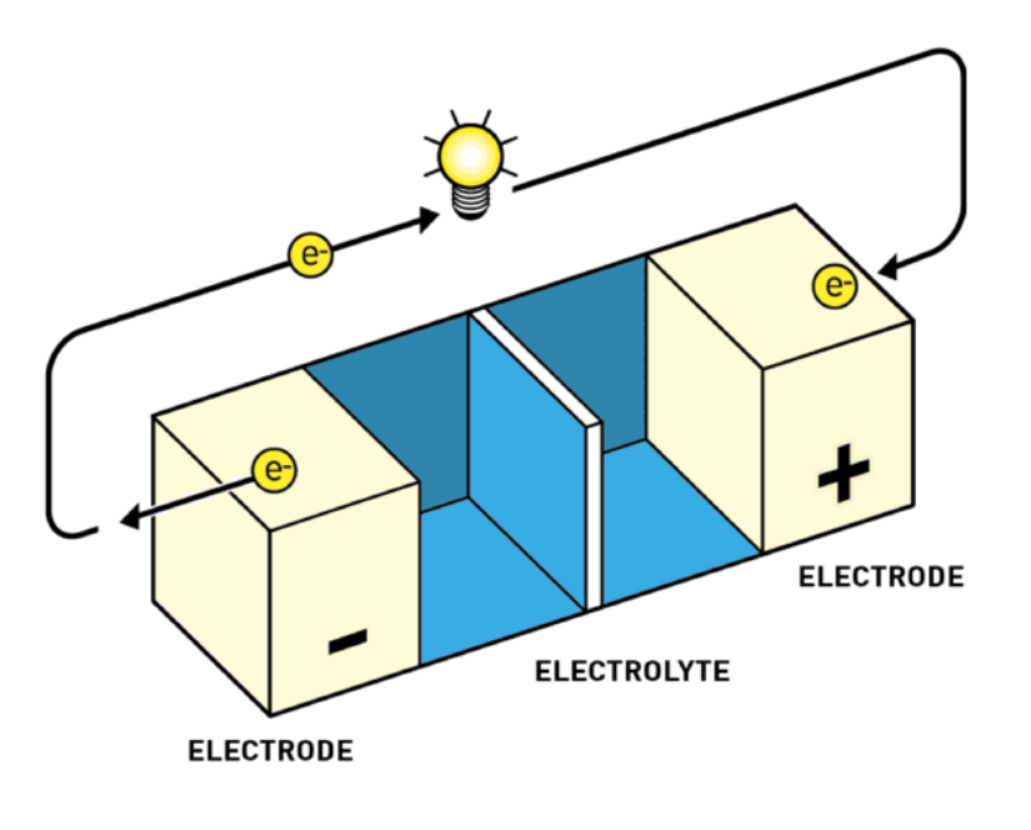
\includegraphics[width=0.4\textwidth]{batt_func_ppr.png}
    \end{center}
    \caption{Diagrama del principio básico de funcionamiento de una bateria en el
    proceso de descarga.}
    \label{batt_wk_ppl}
\end{figure}

\noindent En base a este principio de funcionamiento, surgen una gran variedad
de tecnologías, partiendo de la pila voltaica, hecha de dos discos de metales
distintos, uno de zinc y otro de cobre o plata, separados por un dieléctrico
(como cartón o cuero) sumergido en una solución electrolítica.  Durante la
operación, el disco de zinc actua como ánodo, liberando electrones al circuito y
produciendo iones de metal (proceso de oxidación), mientras que la reacción en
el electrodo opuesto depende de las condiciones de trabajo. En presencia del
aire, el metal de cobre es parcialmente oxidado a CuO, y la reducción de CuO a
Cu se da en el electrodo. En la ausencia de aire, los protones en el electrolito
son reducidos a hidrógeno en la superficie del cobre. El voltaje de la celda es
de aproximadamente 0.8-1.1V, dependiendo de la exposición al aire.
Esencialmente, la pila voltaica fue una batería no recargable.

\noindent Despues surgieron las baterías de plomo-ácido, que tiene un principio
de funcionamiento similar a las baterías voltaicas expuestas al aire, pero con
la posibilidad de ser recargadas. Esta tecnología se basa en dos electrodos de
plomo, donde uno se encuentra parcialmente oxidado a oxido de plomo
($\mathrm{PbO_2}$), separado por acido sulfurico que contiene un electrolito.
Durante el proceso de descarga, ocurre un proceso de oxidacion en el electrodo
de plomo (anodo), produciendo electrones, protones y sulfato de plomo
($\mathrm{PbSO_4}$), mientras que el oxido de plomo es reducido a
$\mathrm{PbSO_4}$ en el cátodo. En este caso, el potencial de una celda es de
alrededor 2V.

\noindent Otro logro en el desarrollo de baterías, ocurrió en el 1899 cuando se
desarrolló la primer batería de niquel-hierro (Ni-Fe) y niquel-cadmio (Ni-Cd) o
tambien conocidas como baterias alcalinas, que fueron predecedoras del híbrido
niquel-metal (Ni-MH) que fue comercializada en 1898.

\noindent Las baterías anteriores son basadas en soluciones acuosas, y la
densidad energetica de las mismas no es alta, especificamente son menores a los
100Wh/kg. Para incrementar la densidad energética de estas baterías, es
necesario encontrar una estabilidad electroquímica del agua ya que juega un rol
muy importante en ello. Además, cuando ambos electrodos utilizando el alto
potencial del plomo, el voltaje de salida solo puede alcanzar un máximo de 2.2V.
Como resultado, con la necesidad de incrementar la densidad energética de una
celda, se descubrio el metal de litio y su aplicacicación en las celdas que
llevan su nombre.

\subsubsection{Litio}

El litio es un metal descubierto en 1818 que tiene excelentes propiedades para
servir como material para el desarrollo de baterías.  Es el metal mas liviano
con una densidad de 0.53$\mathrm{g/cm^3}$.  Tambien tiene un potencial de
reduccion muy bajo, que lo hace ideal para celdas de alta densidad y alto
voltaje. Sin embargo, es un metal reactivo que debe ser protegido, por ejemplo,
del agua y del aire, ya que el contacto con estos provoca que el mismo sea muy
complicado de dominar, imposibilitando su uso para la aplicación deseada.  Esta
protección al medio no es trivial, y factores, tales como su caracter inerte,
punto de fusión, la estabilidad del \emph{redox}, solubilidad de iones de litios
y sales, velocidades de transferencia ion/electrón, viscosidad, entre otros
deben ser considerados.

\noindent Las primeras baterías de litio alcanzaron el mercado en 1970 y la
comercialización de las mismas comenzó en Japón en el año 1991, cuando
\emph{Sony Corporation} presentó el primer modelo.

\noindent Las baterías de litio-ion son definidas en \cite{def_liion} como
almacenadores de energía que utilizan iones de Litio como portadores de carga.
En base a esta definición, el término \emph{batería de Litio-Ion} no se
corresponde con una sola composición química, como lo son las baterías de ácido
o niquel-cadmio, si no que expresa una familia de baterías que dependen de los
iones de Litio pero que pueden ser conformadas por distintos materiales.

\noindent A diferencia de las baterías de ácido, hay dos razones principales por
las cuales las baterías de Litio-ion han crecido en popularidad en tan poco
tiempo: su excelente rendimiento y la capacidad de adaptarse al creciente
mercado de la electrónica de consumo, como por ejemplo, videograbadoras,
celulares y computadoras. A partir de la primer década del siglo XXI, se
comenzaron a utilizar en vehículos eléctricos, como también en grandes sistemas
de almacenamiento de energía, capaces de alimentar barrios residenciales
enteros.

\noindent Desde el 2000 al presente, se desarrollaron varios tipos de baterias
basadas en el litio. Entre ellas se encuentran las baterias de litio-sulfuro
(Li-S) y litio-aire (Li-air), cuya densidad energética teórica ronda los 2600
Wh/kg y 11400 Wh/kg, repectivamente. En 2012, se desarrolló una bateria de
litio-ion recargable acuosa o \acrshort{ARLB} (del ingles
\emph{\acrlong{ARLB}}), que utiliza metal de litio recubierto como ánodo en una
solución de electrolitos mejorando ampliamente la densidad energética.

\subsubsection{Principio de funcionamiento}

El principio de los procesos de carga y descarga en las baterías de litio-ion se
basan en utilizar óxido de litio-cobalto ($\mathrm{LiCoO_2}$) y grafito como
típicos materiales de electrodo. La Figura \ref{op_lithium-ion} ilustra el
princio de operación, y las reacciones de los electrodos se expresan en  las
Ecuaciones \ref{li_anode}, \ref{li_catode} y \ref{li_total}

\reaction{\text{Electrodo positivo: } LiCoO2 <=>[Carga][Descarga] Li_{1-x}CoO2 + xLi + xe^- \label{li_anode}}
\reaction{\text{Electrodo negativo: }6C + xLi^+ + xe^- <=>[Carga][Descarga] Li_{x}C6 \label{li_catode}}
\reaction{\text{Reaccion total: }6C + LiCoO2 <=>[Carga][Descarga] Li_{x}C6 + Li_{1-x}CoO2 \label{li_total}}

\noindent El \ce{LiCoO2} tiene una estructura reticular octaedrica con un
arreglo alternativo de capas de \ce{Li+} y \ce{Co^{3+}}. Durante el proceso de
carga, los iones de litio (en estado iónico) se desintercalan de la estructura
de capas del material del electrodo positivo, liberando electrones, al mismo
tiempo, el \ce{Co^{3+}} se oxida convirtiendose en \ce{Co^{4+}}.  Por el otro
lado, durante el proceso de descarga, con la intercalación de \ce{Li+} dentro de
la reticula, el \ce{Co^{4+}} es reducido a \ce{Co^{3+}}, ganando electrones,
ademas se obtienen electrones de la reticula para convertirse en litio en estado
atómico. Durante este proceso, el estado atómico del litio pierde electrones
convirtiendose en iones de litio , este proceso se puede resumir en que el ánodo
provee al electrodo positivo iones de litio. Dado que el litio se mueve entre el
electrodo positivo y negativo hacia ambos lados a este tipo de baterías se las
denomina, como una batería mecedora (del ingles, \emph{rocking chair}).

\begin{figure}[h!]
    \begin{center}
	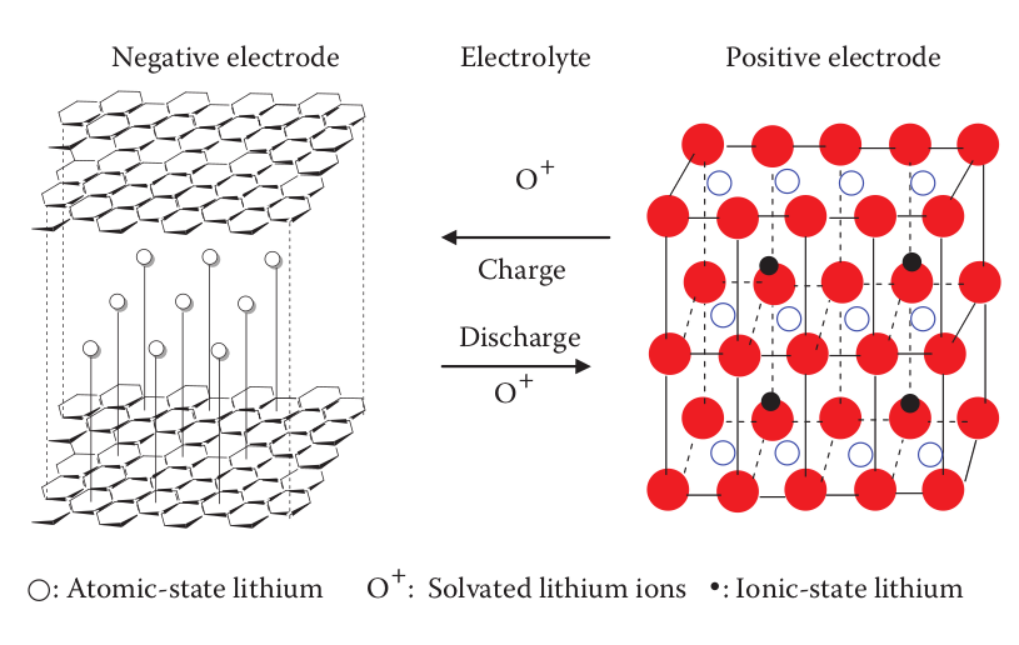
\includegraphics[width=0.7\textwidth]{prin_litio}
	\caption{Esquematico del prinicipio de operacion de una bateria de
	litio-ion.}
	\label{op_lithium-ion}
    \end{center}
\end{figure}

\noindent La mayoría de estas baterías usan materiales de carbón, tales como el
grafito y el carbón duro como ánodo. Otros utilizan óxidos de metales, como por
ejemplo, el Titanato de Litio ($\mathrm{Li_4Ti_5O_{12}}$) y el Pentóxido de
Niobio ($\mathrm{Nb_2O_5}$), debido a que pueden aceptar iones de Litio cuando
son cargados, y liberarlos en el proceso de descarga, estas reacciones se
denominan como inserción y extracción respectivamente.  Los potenciales de
reacción de estos materiales son mucho más bajos que los electrodos de hidrógeno
estándares, por lo tanto, el electrolito debería ser estable inclusive para
niveles de potencial tan bajos. Ésta es la razón por la cual, los electrolitos
orgánicos, que consisten de solventes orgánicos y sales de litio, son utilizados
en las baterías de Litio-ion en vez de electrolitos acuosos.

\noindent El material activo del cátodo debe contener Litio en su composición
química para proveer una fuente de iones de Litio. Durante la primer etapa de
desarrollo de las celdas de litio, se utilizaba Óxido de Litio-Cobalto.  También
se estudió el uso de $\mathrm{LiNiO_2}$ como material activo para el cátodo pero
fue inmediatamente descartado debido a su inestabilidad térmica. Sin embargo, se
desarrollaron y utilizaron derivativos de esta composición, formulados como
$\mathrm{LiM_xNi_{1-x}O_2}$ (M: elemento metálico tales como, el Co, Mn, Al,
Mg).

Comparada con las baterías de litio-ion originales en los principios de 1990, el
rendimiento de las mismas ha sido mejorado de forma significativa con el paso
del tiempo. Los últimos desarrollos tienen ventajas dominantes sobre las
baterías recargables tradicionales:

\begin{itemize}
    \item \textbf{Alta densidad energética:} La densidad energética por
	volumen y masa para una batería de litio modelo 18650 puede alcanzar
	los 500 Wh/$\mathrm{dm^3}$ y 230 Wh/kg, respectivamente, que ademas
	se encuentra en continuo aumento a medida que se investigan y
	desarrollan nuevas tecnologías.
    \item \textbf{Alto voltaje de salida (~3.6V):} Esto es 3 veces mayor a
	las baterías recargables de Ni-Cd o Ni-MH.
    \item \textbf{Alta potencia de salida:} Pueden alcanzar hasta 2kW/kg for
	un corto periodo de tiempo.
    \item \textbf{Baja auto-descarga:} La descarga media de las celdas de
	litio son menores a un 3\% mensuales, que es la mitad que las celdas
	basadas en Ni-Cd y Ni-MH.
    \item \textbf{Bajo efecto de histéresis} A diferencia de las celdas de
	Ni-Cd y Ni-MH las celdas de litio tienen un efecto de histéresis
	despreciable con el paso de los ciclos de carga-descarga de la
	misma, resultando en un mejor ciclo de vida con respecto a los otros
	tipos de celdas.
    \item \textbf{Ciclos de carga-descarga rápidos:} Las baterías de
	litio-ion pueden ser cargadas con corrientes de hasta un 80\% de su
	capacidad. Es decir, si la batería tiene una capacidad de 3Ah, la
	misma se puede cargar a una corriente de 3A.
    \item \textbf{Alta eficiencia culombica:} La eficiencia culombica o EC,
	es un parametro que permite obtener que porcentaje del material
	activo se convierte en energia. Su medicion es importante porque 
	permite medir el desempeño de la bateria con respecto a otras 
	tecnologias. En el caso de las celdas de Litio-ion, la eficiencia 
	culombica se mantiene casi en un 100\% inclusive despues del primer
	ciclo.
    \item \textbf{Gran rango de temperaturas}: Las baterias de litio-ion
	pueden operar entre -25\degree C a +45\degree C. Las
	investigaciones actuales quieren extender ese rango desde
	-40\degree C a +70\degree C con mejoras en el
	electrolito y los materiales de los electrodos.

	Esto depende fuertemente del 
	alto voltaje, porque la energía específica es el producto del voltaje 
	de la celda y su capacidad específica, lo que hace que las celdas de 
	Litio-Ion se destaquen a comparación de otras tecnologías, 
	como por ejemplo, las celdas de Niquel-metal con un voltaje de 1.2V 
	pero con mayor capacidad tienen menor energía específica. 
    \item \textbf{Alta eficiencia energética:} Esto se debe a dos 
	factores principales, por un lado se debe a la alta eficiencia de 
	carga y descarga debido a que no hay pérdidas durante las reacciones 
	químicas de la celda en ambos procesos y, nuevamente, esto se atribuye 
	también a su alto voltaje. Éste último, se debe a que la eficiencia 
	energética, es el restante de la tensión operativa en relación a la 
	tensión en circuito abierto. Suponiendo que tenemos una celda A con una 
	tensión de circuito abierto ($\mathrm{V_A}$) mayor que otra celda B con 
	una tensión $\mathrm{V_B}$, que tiene la misma pérdida de voltaje X, 
	la eficiencia de A va a ser mayor que la de B, dado por:
	\vspace{5mm}
	\begin{equation}
	    \frac{V_A - X}{V_A} > \frac{V_B - X}{V_B} \nonumber
	\end{equation}
    \item \textbf{Larga duración:} Esto se atribuye a que las reacciones 
	dentro de la celda, durante los ciclos de carga y descarga, no realizan 
	cambios morfológicos significativos. Esto es bastante distinto con las 
	baterías de ácido, donde la reacción que se lleva a cabo involucra la 
	disolución y deposición de materiales, lo que representa grandes 
	cambios morfológicos durante los ciclos de carga y descarga.
\end{itemize}

\noindent Por último, las baterías de Litio-ion utilizan electrolitos orgánicos.
El electrolito permite que la celda tenga alto niveles de tensión, sin embargo
la combustibilidad del mismo genera problemas de seguridad. Por lo tanto, es
clave para el desarrollo de estas baterías minimizar la causa y efecto de la
combustión de la misma sin sacrificar rendimiento.

\begin{figure}[h!]
    \begin{center}
	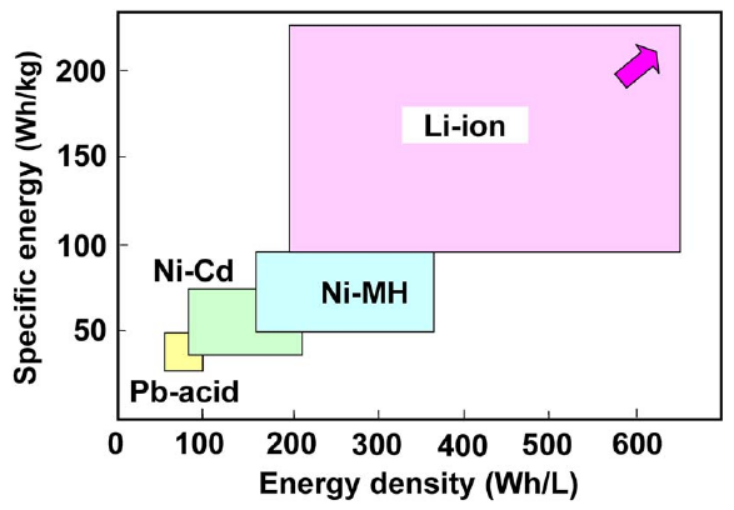
\includegraphics[width=0.6\textwidth]{comparisson-liion.png}
	\caption{Grafica comparativa entre distintas
	tecnologías de baterías.}
	\label{comparisson_batt}
    \end{center}
\end{figure}
\FloatBarrier

\noindent El estado de las baterías de Litio-ion con respecto a las otras
tecnologías se puede observar en la Figura \ref{comparisson_batt}, donde se
puede observar la dominancia de las mismas sobre el resto de las tecnologías, en
términos de densidad energética (Wh/L) y energía específica (Wh/kg). La flecha
de la esquina derecha indica que ésta tecnología se encuentra en constante
desarrollo y puede mejorar con el paso del tiempo.

\noindent La aplicación práctica de las baterías de Litio-ion involucra la
integración de las mismas dentro de un sistema, involucrando un controlador
central (\acrshort{BMS}), sistemas de refrigeración, sensores y conectores entre
las celdas. En este sistemas las celdas pueden conectarse de distintas formas,
por ejemplo, pueden conectarse en paralelo, para incrementar la capacidad del
pack, en serie, para incrementar el voltaje, o combinadas para lograr ambos
cometidos al mismo tiempo. Por ejemplo, un auto eléctrico de la marca
\emph{Tesla}, posee un pack de baterías de 85KWh compuesto por 7104 celdas, con
una arquitectura de 16 módulos conectados en serie , donde cada uno posee 444
celdas conectadas en paralelo.

\subsubsection{Batería Seleccionada}\label{batSel}

\noindent En este caso utilizaremos celdas de Litio-ion modelo NCR18650PF,
integrando una arquitectura \emph{6S3P}, es decir, 6 modulos conectados en serie
donde cada uno esta compuesto por 3 celdas conectadas en paralelo.  En la Figura
\ref{pack} se muestra el esquemático de la arquitectura del pack como también
una foto de la celda que se utilizará para conformar el pack. 

\begin{figure}[h!]
    \begin{subfigure}[b]{.5\textwidth}
	\begin{center}
	    \begin{minipage}[c]{0.45\textwidth}
		\centering
		\begin{circuitikz}[european]

		    \draw (7, 2) -- (7, 2.2);
		    \draw (7, 2) to[battery1] (7, 1.6);
		    \draw (7, 1.4) -- (7, 1.6);
		    \draw (7, 1.4) to[battery1] (7, .9);			
		    \draw (7, .7) -- (7, .9);			
		    \draw (7, 0.7) to[battery1] (7, 0.2);			
		    \draw (7, 0.2) -- (7, -0.2);
		    \draw (7, -0.2) to[battery1] (7, -0.7);
		    \draw (7, -.7) -- (7, -.9);
		    \draw (7, -.9) to[battery1] (7, -1.4);
		    \draw (7, -1.4) -- (7, -1.6);
		    \draw (7, -1.6) to[battery1] (7, -2);
		    \draw (7, -2) -- (7, -2.2);

		    \draw (9, 2) -- (9, 2.2);
		    \draw (9, 2) to[battery1] (9, 1.6);
		    \draw (9, 1.4) -- (9, 1.6);
		    \draw (9, 1.4) to[battery1] (9, .9);			
		    \draw (9, .7) -- (9, .9);			
		    \draw (9, 0.7) to[battery1] (9, 0.2);			
		    \draw (9, 0.2) -- (9, -0.2);
		    \draw (9, -0.2) to[battery1] (9, -0.7);
		    \draw (9, -.7) -- (9, -.9);
		    \draw (9, -.9) to[battery1] (9, -1.4);
		    \draw (9, -1.4) -- (9, -1.6);
		    \draw (9, -1.6) to[battery1] (9, -2);
		    \draw (9, -2) -- (9, -2.2);

		    \draw (11, 2) to[battery1] (11, 1.6);
		    \draw (11, 1.4) -- (11, 1.6);
		    \draw (11, 1.4) to[battery1] (11, .9);			
		    \draw (11, .7) -- (11, .9);			
		    \draw (11, 0.7) to[battery1] (11, 0.2);		
		    \draw (11, 0.2) -- (11, -0.2);
		    \draw (11, -0.2) to[battery1] (11, -0.7);
		    \draw (11, -.7) -- (11, -.9);
		    \draw (11, -.9) to[battery1] (11, -1.4);
		    \draw (11, -1.4) -- (11, -1.6);
		    \draw (11, -1.6) to[battery1] (11, -2);
		    \draw (11, -2) -- (11, -2.2);

		    \draw (7, 0) -- (9, 0);
		    \draw (9, 0) -- (11, 0);

		    \draw (7, 0.8) -- (9, 0.8);
		    \draw (9, 0.8) -- (11, 0.8);

		    \draw (7, 1.5) -- (9, 1.5);
		    \draw (9, 1.5) -- (11, 1.5);

		    \draw (7, 2.2) -- (9, 2.2);
		    \draw (9, 2.2) -- (11, 2.2);			

		    \draw (7, -0.8) -- (9, -0.8);
		    \draw (9, -0.8) -- (11, -0.8);

		    \draw (7, -1.5) -- (9, -1.5);
		    \draw (9, -1.5) -- (11, -1.5);

		    \draw (7, -2.2) -- (9, -2.2);
		    \draw (9, -2.2) -- (11, -2.2);			

		    \draw [dashed] (6.5, 2.4) rectangle (11.5, -2.4);

		    \draw node at (8.2, 2.6) {Pack de Baterías 6s3p};
		\end{circuitikz}
	    \end{minipage}
	\end{center}
	\caption{Esquemático de la arquitectura del pack de baterías.}
	\label{pack_bateria}
    \end{subfigure}%
    ~
    \begin{subfigure}[b]{.45\textwidth}
	\centering
	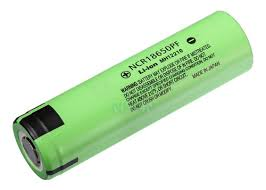
\includegraphics[width=0.7\textwidth]{18650.jpg}
	\caption{Foto celda NCR18650PF.}
	\label{foto_bateria}
    \end{subfigure}
    \caption{Pack 6s3p y Celda NCR18650PF.}
    \label{pack}
\end{figure}
\FloatBarrier

Estas celdas se caracterizan por su cátodo, cuya composición química se basa en
el óxido de Litio Niquel Cobalto Aluminio ($\mathrm{LiNiCoAlO_2}$) y, según su
hoja de datos \cite{18650_datasheet}, sus carateristicas electricas se pueden
observar en la Tabla \ref{table:ncr}.  \newpage

\begin{table}[h]
    \begin{center}
	\begin{tabular}{|c|l|}
	    \hline
	    \multicolumn{2}{|c|}{Especificaciones elecctricas}                          \\ \hline
	    \textbf{Capacidad Específica}                 & 2700mAh                            \\ \hline
	    \multirow{2}{*}{\textbf{Capacidad}}           & Mínimo: 2750mAh                    \\ \cline{2-2} 
	    & Tipico: 2900mAh                    \\ \hline
	    \textbf{Corriente de Descarga Máxima}         & 10000mAh($\sim$3.5C)               \\ \hline
	    \textbf{Rango operativo de tensión}           & 2.5V - 4.2V                        \\ \hline
	    \textbf{Voltaje Nominal}                      & 3.6V                               \\ \hline
	    \textbf{Charga}                               & CC-CV, Std. 1375mA, 4.20V, 4.0 hrs \\ \hline
	    \textbf{Peso}                                 & 48g                              \\ \hline
	    \multirow{3}{*}{\textbf{Temperatura}}         & Carga: 0 a 45C                     \\ \cline{2-2} 
	    & Descarga: -20 a 60C                \\ \cline{2-2} 
	    & Almacenaje: -20 a 50C              \\ \hline
	    \multirow{2}{*}{\textbf{Densidad Energética}} & Volumetrica: 577Wh/l               \\ \cline{2-2} 
	    & Gravimetrica: 207wh/kg             \\ \hline
	\end{tabular}%
	\caption{Especificaciones electricas de una celda de litio NCR18650PF}
	\label{ncr_table}
    \end{center}
    \caption{Especificaciones elecctricas - Panasonic NCR18650PF}
    \label{table:ncr}
\end{table}

Por el otro lado, la hoja de datos también nos provee curvas significativas,
como por ejemplo, la curva de carga \emph{(Fig. \ref{cc_cv_18650})}, la curva de
descarga para distintas corrientes \emph{(Fig. \ref{descarga_18650})} y la curva
del ciclo de vida típico de la batería \emph{(Fig. \ref{life_cycle_18650})}.

\begin{figure}[h!]
    \begin{subfigure}[t]{.5\textwidth}
	%   		\centering
	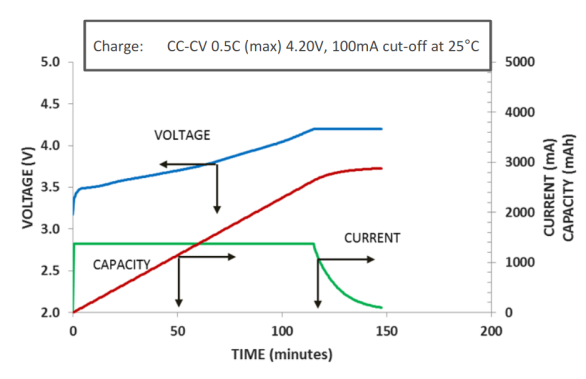
\includegraphics[width=1\textwidth]{cc_cv_18650.png}
	\caption{Curva de carga.}
	\label{cc_cv_18650}
    \end{subfigure}%
    ~ 
    \begin{subfigure}[t]{.5\textwidth}
	%    		\centering
	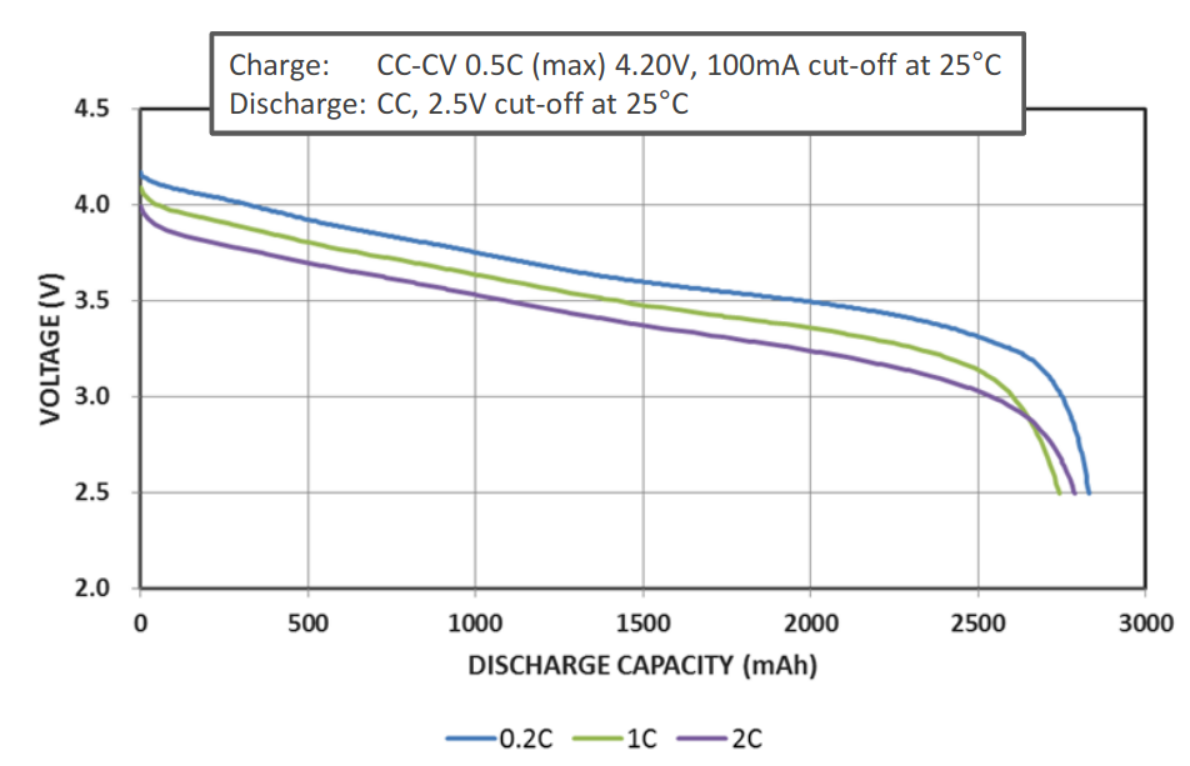
\includegraphics[width=1\textwidth]{discharge_18650.png}
	\caption{Curva de descarga en base a distintas corrientes de descarga (0.5C,
	1C, 1.5C y 2C)}
	\label{descarga_18650}
    \end{subfigure}
    ~ 
    \begin{centering}
	\begin{subfigure}[t]{1\textwidth}
	    \centering
	    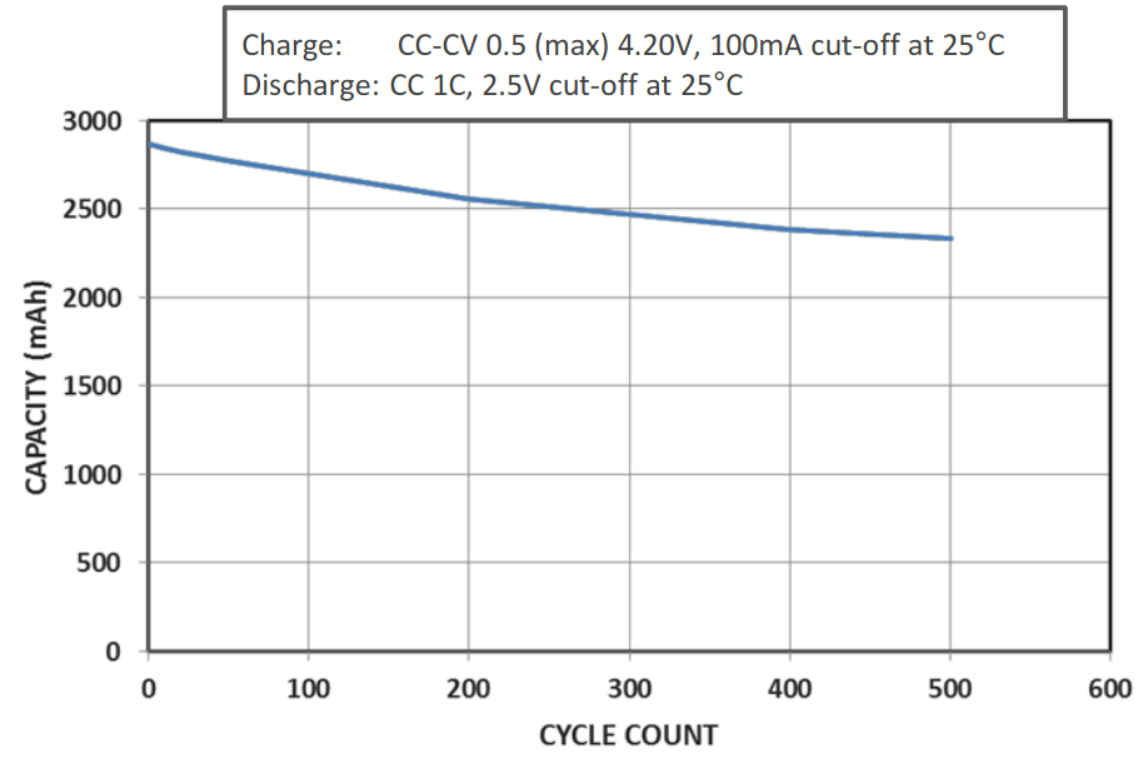
\includegraphics[width=0.5\textwidth]{life_cycle_18650.png}
	    \caption{Curva del ciclo de vida de una celda 18650}
	    \label{life_cycle_18650}
	\end{subfigure}
    \end{centering}
    \caption{Curvas sgnificativas celda Panasonic 18650PF}
    \label{curvas_sign_18650}
\end{figure}

\newpage 

\subsection{Sensado de Corriente}

El sensado de la corriente de carga como de descarga del pack de batería juega
un rol muy importante en el desarrollo exitoso de un \acrshort{BMS}. Es a partir
de conocer con precisión la magnitud de corriente que el sistema podrá mantener
el pack de baterías operando dentro de la zona segura (\acrshort{SOA} por sus
siglas en ingles), monitorear la distribución de carga entre las celdas,
implementar correctamente los algoritmos de ecualización de carga y mantener un
seguimiento preciso del estado de carga.

\noindent Existen en el mercado una gran variedad de tecnologías y 
soluciones para la medición de corriente en las diferentes aplicaciones. 
Algunas de las tecnologías mas relevantes, disponibles en el mercado son:
\begin{itemize}
    \item Resistencia Shunt
    \item Transformadores de intensidad (TI)
    \item Bobina de Rogowski 
    \item Sensores de Efecto Hall
    \item Sensores de Impedancia Magnética (MI)
    \item Sensores de Magnetoresistencia Gigante 
    \item Sensores Ópticos (Experimental)
\end{itemize}

Dentro del amplio abanico de métodos y tecnologías utilizadas para la medición
de corrientes los dos más elegidos e implementados en Sistemas de Administración
de Baterías \acrshort{BMS} son las mediciones a partir de resistencias Shunt y
mediciones a partir de sensores de efecto hall.

\subsubsection{Resistencia Shunt}

La tecnología Shunt se vale del Sensado de la caída del voltaje sobre una
resistencia de unos pocos mili ohmios en serie con el paso de la corriente
incógnita para la medición indirecta de la corriente.

El método de sensado por resistencia tipo shunt presenta una de las mejores
relaciones costos-efectividad, presentando un empaquetado compacto y aplicable
en mediciones de corrientes tanto continua como alterna encontrando su
frecuencia de corte por encima de las decenas de Mhz.

Las mediciones por resistencia shunt carecen naturalmente de aislación galvánica
debiendo ser resuelta a partir del circuito de implementación. Generalmente, los
shunts presentan bajo coeficiente de temperatura de resistencia, (\acrfull{TCR}
por sus siglas en ingles). Característica fundamental en las implementaciones de
\acrshort{BMS} en sistemas de vehículos eléctricos que permite aumentar el rango
de temperatura de operación del sistema.

Aunque los shunts de corrientes operen bajo el principio de caida de voltaje
ohmico, en la práctica las resistencias presentan una inductancia intrínseca que
comprometen la precisión y el ancho de banda máximo de las mediciones.

\subsubsection{Sensor de efecto Hall}

El sensor de efecto Hall es un sensor de efecto magnético basado en el fenómeno
físico homónimo que le da su nombre.  El sensor de efecto Hall es un dispositivo
aislado, no intrusivo que puede ser utilizado para medir corriente tanto
continua como alterna de hasta unos cientos de kHz. El sensor Hall puede ser
fabricado utilizando tecnología CMOS convencional pero a un costo mayor que las
implementaciones con transformadores de corriente o bobinas de Rogowski.

El traductor de efecto Hall encuentra normalmente su límite de medición en los
picos de corriente debido al fenómeno de saturación magnética del núcleo y
encuentra su límite de ancho de banda en las frecuencias menores al MHz. A su
vez, esta tecnología es sumamente sensible a la influencia de los campos
magnéticos externos. Frente a estas limitaciones es común que los sensores de
efecto Hall se implementen mayoritariamente con bobinas cerradas para lograr una
mejor precisión y un rango mayor de operación dinámico.

El voltaje de offset presente en la medición del dispositivo es poco estable y
varia fuertemente frente a las variaciones de temperatura de operación.

\begin{figure}[h!]
    \centering
    \begin{subfigure}[b]{0.4\linewidth}
	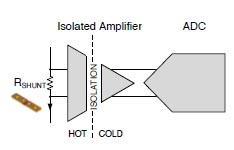
\includegraphics[width=\linewidth]{../assets/R-Shunt_Isolated_Sensor.jpg}
	\caption{Sensado por Resistencia Shunt}
    \end{subfigure}%
    \hspace{15mm}
    \begin{subfigure}[b]{0.4\linewidth}
	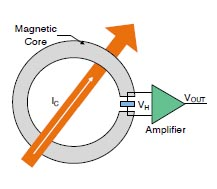
\includegraphics[width=\linewidth]{../assets/Open-loop_Hall_Sensor.jpg}
	\caption{Sensado por efecto Hall de loop abierto}
    \end{subfigure}
    \caption{Diagramas - Métodos de sensado de corriente}
    \label{fig:SenseMetods}
\end{figure}

\subsubsection{Tecnología Seleccionada}

Frente a los requerimientos y la naturaleza de un \acrshort{BMS} hemos
seleccionado la tecnología de sensado de corriente por resistencia Shunt.
Actualmente existen en el mercado un sin número de soluciones de amplificadores
y moduladores aislados que permiten alcanzar precisas mediciones de corrientes
con este método logrando minimizar las injerencias del entorno siempre y cuando
se seleccione una resistencia Shunt adecuada.

\noindent Las ventajas de la medición a partir del método de resistencia 
shunt son:

\begin{itemize}
    \item Bajo offset y baja susceptibilidad frente a influencias de campos 
	magnéticos externos y variaciones de temperatura.
    \item Alta linealidad de la solución en todo el rango de voltaje en 
	comparación a la solución basada en tecnología Hall, sobre todo en 
	la zona cercana a cero y la de saturación del nucleo. 
    \item Mejor resolución para mediciones de corriente continua frente a 
	las soluciones basadas en mediciones de efecto Hall. 
	Particularmente debido a la baja sensitividad que presenta frente a 
	las influencias de los campos magnéticos externos.
    \item Pueden soportar operaciones en ambientes de altas temperaturas 
	manteniendo la linealidad debido a su bajo TCR. 
	Los sensores de efecto Hall encuentran su rango de operación 
	fuertemente acotado.
    \item Facilidad que presenta la tecnología para la integración en 
	circuitos impresos priorizando el tamaño reducido.
    \item Disponibilidad en distribuidores nacionales
\end{itemize}

\noindent El integrado propuesto para el sensado de corriente es el INA226 de
Texas Instruments. El INA226 es un conversor analógico digital de 16 bits (ADC)
que implementa una interfaz compatible I2C para la comunicación con el módulo
del control. El dispositivo monitorea simultaneamente la tensión que cae en una
resistencia shunt y la del bus de alimentación. Permite múltiples calibraciones
y seteos, entre ellos variar los tiempos de conversión y definir conversiones
múltiples que al implementar internamente un multiplicador y divisor permite
obtener lecturas directas de tensión y potencia en amperes y en Vatios.

Observamos en la figura \ref{fig:ina226-commonimplementation} su implementación
modelo. 

\begin{figure}[h!]
    \begin{center}
	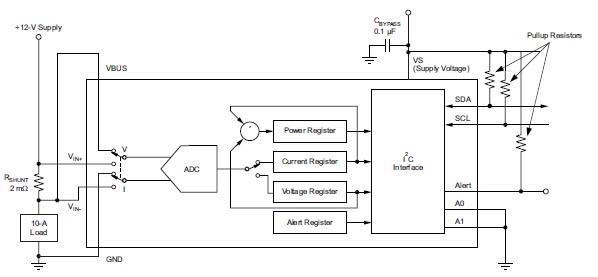
\includegraphics[width=0.7\linewidth]{assets/INA226-Common_Implementation}
	\caption{Implementación Tipo - INA226}
	\label{fig:ina226-commonimplementation}
    \end{center}	
\end{figure}
\FloatBarrier

\subsection{Algoritmos de Estimación del Estado de Carga}

La estimación del estado de carga es una de las tareas fundamentales dentro del
sistema de Administración de baterías ya que en base a esta información se toman
importantes decisiones, de ella dependen la optima ecualización de carga de las
celdas, no exceder los límites de Zona de Operación segura, realizar acciones
preventivas en caso del agotamiento de carga como ser iniciar un apagado de
seguridad y por último reportar al usuario la carga restante en el pack.

A priori hay 2 métodos básicos de estimación de carga, el primero,
\textbf{\emph{OCV vs SoC}}, aprovecha la relación entre el Estado de Carga SoC
(del ingles \acrfull{SOC}) y el voltaje de circuito abierto o OCV (del ingles
\acrfull{OCV} éste método es económico pero tiene 2 principales desventajas, la
curva OCV vs SoC tiene una región en la cual tiene valores de pendiente
despreciable lo que genera que entre el 80\% de carga y el 35\% aproximadamente,
haya solo unas pocas decenas de milivoltios de diferencia. Debido a esto un
error de pocos milivolts genera grandes diferencias en la estimación de la carga
real. Por otro lado la estimación mediante voltaje tiene problemas a la hora de
determinar el voltaje online, es decir cuando la batería esta conectada a una
carga las corrientes que circulan por el pack generan caidas de tensión debido a
las impedancias internas del pack, si estas no son tenidas en cuenta pueden
llevar a que el ecualizador del pack desbalancee aún más el pack.

El segundo método es el \textbf{\emph{Conteo de carga}} o \textbf{\emph{Coulomb
Counting}}, el mismo consiste en integrar la corriente a lo largo del tiempo
obteniendo así la carga total en el pack o SoC mediante la ecuación
\ref{SOC_Coulomb_C}, donde \emph{i} corresponde a la corriente de la batería y
$C_\eta$ la capacidad nominal de la misma.

\begin{equation}
    SOC=1-\frac{\int{i.dt}}{C_\eta}
    \label{SOC_Coulomb_C}
\end{equation}	

Este método funciona muy bien en la zona donde el primer método falla, sin
embargo como todo proceso de integración, genera errores iterativos en cada
ciclo de cálculo generando que a lo largo del tiempo el error absoluto de este
método tienda a crecer.Además de la necesidad de establecer un valor inicial de
carga, estos puntos de referencia pueden ser la carga total de la batería o la
máxima profundidad de descarga o DOD (de sus siglas en ingles \acrfull{DOD} ) de
manera que exigen a la batería llegar a puntos límites de carga disminuyendo su
vida útil.

Debido a que nos interesa saber el \acrshort{SOC} cuando la batería esta
entregando energía o siendo cargada se deben tener en cuenta los principales
factores que afectan a la estimación de carga on-line. Un modelo utilizado para
relacionar la tensión entre los bornes de la batería y el \acrshort{OCV}
utilizado con gran frecuencia es el modelo eléctrico bosquejado en la \emph{Fig.
\ref{Electric_model}}, este modelo es coherente con el hecho de que la tensión
en los bornes de la batería en reposo es igual al \acrshort{OCV}. Pero al ser
circulada por una corriente se deben tener en cuenta los fenómenos dinámicos  y
la perdida por resistencias internas así como la corriente de pérdida (auto
descarga) de la batería.

\begin{figure}[h!]
    \begin{center}
	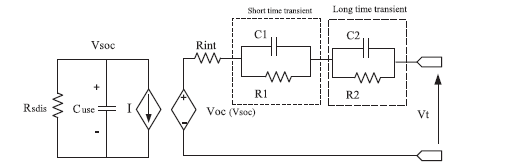
\includegraphics[width=0.7\textwidth]{electric_battery_model_2_order.png}
	\caption{Modelo Electrico de segundo orden con corriente de perdida.}
	\label{Electric_model}
    \end{center}
\end{figure}

Dada la naturaleza química de la batería, si se entra en detalle se puede
observar que los componentes que modelan la batería tienen un comportamiento no
lineal dependiendo del \acrshort{SOC} y más aún se ven afectados por el efecto
de envejecimiento de las celdas, es decir, estamos es un sistema no lineal no
estacionario.

Como soluciones parciales fueron desarrollados varios métodos los cuales son una
solución de compromiso entre aproximaciones lo suficientemente conservadoras
para obtener el menor error posible y un alto costo computacional cuyas
exigencias de hardware elevan el costo y el espacio necesario para su
implementación, clasificándose según \cite{Hannan2017} los siguientes métodos
como convencionales :

\begin{itemize}
    \item Fuerza Electro-Motriz
    \item Estimación basada en modelos (Térmico y electroquímicos)
    \item Resistencia interna
    \item Espectroscopia Dieléctrica
\end{itemize}

Un gran avance en la estimación del estado de carga fue la aplicación de los
Filtro de Kalman para disminuir el error. Esta es una herramienta estadística de
análisis en espacio de estado que mediante las matrices de Varianza y Covarianza
estiman un vector de soluciones con mayor precisión.  Los Filtros de Kalman ven
afectado su rendimiento a la hora de trabajar con sistemas fuertemente No
Lineales, debido a esto surgen las variantes EKF, UKF y SPKF provenientes del
inglés, Extended, Unscented y Sigma Point, respectivamente.

\subsubsection{Método de estimación por FEM}

Teniendo en cuenta la limitación del método de \acrshort{OCV} para la estimación
mientras la batería esta siendo cargada o descargada, surge como solución a esta
problemática la estimación del \acrshort{OCV} mediante el estudio de la
respuesta temporal de la tensión entre los terminales de la batería dado su
comportamiento temporal regido por una ecuación diferencial de primer orden como
se muestra en \emph{\ref{1er_orden_eq}}, siendo k una constante, cuya solución
es de la forma \emph{\ref{1er_orden_sol}}, lo cual se corresponde con la gráfica
de la \emph{Fig.\ref{EMF_Method}}.

\begin{equation}
    \frac{df(x)}{dx} = \alpha f(x)
    \label{1er_orden_eq}
\end{equation}  

\begin{equation}
    f(x)= x_{(\infty)}+(x_0-x_{(\infty)})e^{-\alpha x}
    \label{1er_orden_sol}
\end{equation}  

\clearpage

\begin{figure}[h]
    \begin{center}
	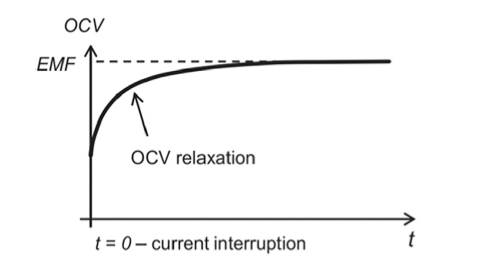
\includegraphics[width=0.7\textwidth]{EMF_Relaxation.png}
	\caption{Curva de relajación de una Batería de Li-Ion}
	\label{EMF_Method}
    \end{center}
\end{figure}

\subsubsection{Estimación basada en modelos (Mecánicos, Térmicos y electroquímicos)}

Este método requiere un profundo conocimiento de los fenomenos físicos y
electroquímicos dentro de las baterías, como por ejemplo la concentración de
electrolito, concentración de material, densidad microscópica de corriente. Esto
constituye su principal desventaja ya que es complejo y la obtención de
parámetros no es trivial para todo tipo de baterías.

Las celdas de Li-Ion se componen de 5 regiones: un electrodo negativo colector
de corriente, un electrodo compuesto poroso de inserción negativo, un separador
poroso, un electrodo compuesto poroso de inserción positivo y un electrodo
positivo colector de corriente. Esto en conjunto con las ecuaciones
\ref{Chrg_cons_hom_sol} - \ref{Butler_Volmer_kinetics} se detalla en
\cite{Li2016}.

%\cite{Li2016}
%Li-ion dynamics and state of charge estimation
%Mingheng Li
%Department of Chemical and Materials Engineering, California State Polytechnic University, Pomona, CA 91768, United States
%el pdf se llama Li2016.pdf en la carpeta xxxx\bms\docs\Bibliography\Papers\SOC Papers

Tomando como modelo un modelo unidimensional a lo largo de la sección de la
batería se aplican las siguentes ecuaciónes:

\vspace{5mm}

Conservación de carga en un sólido homogéneo:

\begin{equation}
    \nabla \cdot (-\sigma\nabla\upvarphi_s)=-j^{Li} 
    \label{Chrg_cons_hom_sol}
\end{equation}	

Conservación de masa en un sólido homogéneo:

\begin{equation}
    \frac{\partial c_s}{\partial t}=\nabla \cdot (D_s\nabla c_s) 
    \label{Mass_cons_hom_sol}
\end{equation}	

Conservación de masa en un electrolito homogéneo:

\begin{equation}
    \varepsilon_e\frac{\partial c_e}{\partial t} + \nabla \cdot (-D_e\nabla c_e) = (\frac{1-t_+^0}{F})j^{Li}
    \label{Mass_cons_hom_electrolyte}
\end{equation}	

Conservación de carga en un electrolito homogéneo:

\begin{equation}
    \nabla \cdot (\upkappa \nabla \upvarphi_e + \upkappa_D \nabla \ln c_e) = -j^{Li}
    \label{Chrg_cons_hom_electrolyte}
\end{equation}	

Ecuación de Butler-Volmer de movimiento de cargas en una unión entre un sólido
conductor y una solución de Iones de Litio con el efecto de doble capa
eléctrica.

\begin{equation}
    j^{Li} = a_si_0[{e^\frac{F\eta}{2RT}-e^{-\frac{F\eta}{2RT}}}]+ a_sC_{dl}\frac{\partial{(\upvarphi_s - \upvarphi_e)}}{\partial t}
    \label{Butler_Volmer_kinetics}
\end{equation}	

En las ecuaciones \ref{Chrg_cons_hom_sol} - \ref{Butler_Volmer_kinetics},
$\sigma$  conductividad de la fase sólida, $\upvarphi_s$ el potencial eléctrico
de la fase sólida, $\upvarphi_e$ el potencial eléctrico del electrolito,
$j^{Li}$ la corriente producida por el consumo de Li, t es el tiempo, c
concentración de Iones de Litio, D el coeficiente de difusión, F la constante de
Faraday, $\varepsilon$ es la fracción por volumen, $t_+^0$ el número de
transferencia, $\upkappa$ la conductividad del electrolito, $\upkappa_D$ la
conductividad de la difusión, $i_0$ la densidad de corriente de intercambio,
$\eta$ la sobretensión, $a$ el area específica and $C_{dl}$ la capacidad de la
doble capa. El subíndice $s$ corresponde a la fase sólida y $e$ corresponde con
el electrolito. También teniendo en cuenta la relación de Bruggerman.

\subsubsection{Estimación por resistencia interna}

Este método utiliza el voltaje y la corriente de la batería en conjunto para
determinar la resistencia interna esta. Durante breves instantes ( menores a 10
ms) se excita la batería con pulso de corriente , asumiendo que este período es
lo suficientemente acotado para no que la variación de tensión sea atribuida a
la resistencia interna y no a la carga/descarga de la batería la resistencia se
obtendría según la formula :

\begin{equation}
    \frac{\Delta V}{\Delta I} = R_\Omega 
    \label{Internal_resistance_EQ}
\end{equation}  

Teniendo en cuenta que si el período del pulso es mayor la medición acumula un
error considerablemente mayor respecto a pulsos breves y teniendo en cuenta que
este método tiene una gran precisión únicamente en valores de SOC cercanos a la
descarga,debido a que varia mucho en este rango, y al bajo valor de las
resistencias (del orden de los miliohm) como se muestra en la \emph{ Fig.
\ref{Internal_resistance}}, extraida de \cite{Hentunen2014}, este método no
termina siendo atractivo debido a las dificultades para obtener valores precisos
de SOC, generando que sea poco utilizado de manera aislada.

%\cite{hentunen2014}
%Time-Domain Parameter Extraction Method for
%Thevenin-Equivalent Circuit Battery Models
%Ari Hentunen, Member, IEEE, Teemu %Lehmuspelto, Member, IEEE, and Jussi Suomela
%el pdf se llama hentunen2014 en la carpeta xxxx\bms\docs\Bibliography\Papers\SOC Papers

\begin{figure}[h]
    \begin{center}
	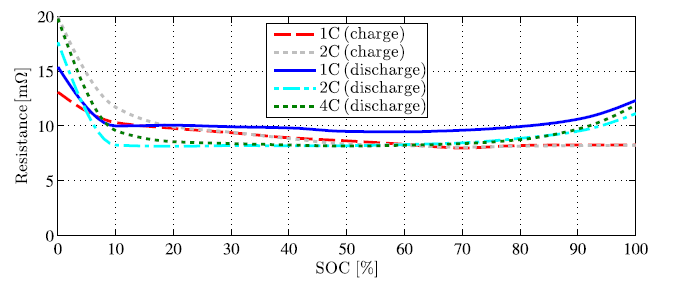
\includegraphics[width=0.7\textwidth]{Ro_vs_SOC.png}
	\caption{Resistencia en Corriente continua de una batería de Li-Ion vs. SOC
	obtenida por HPPC}
	\label{Internal_resistance}
    \end{center}
\end{figure}
\FloatBarrier

\subsubsection{Espectroscopía Dieléctrica (EIS)}

Este estudio consiste en llevar a la celda a un estado de carga conocido, y
luego de un período de relajación se excita los terminales con una onda senoidal
de tensión o corriente y se mide la respuesta de corriente o tensión
respectivamente. En la Fig. \ref{EIS_Nyquist} se observan las curvas obtenidas
por Mingheng Li basadas en un modeló físico basado en principios de conservación
de masa y carga en una interfaz entre un sólido y un electrolito detallado en
\cite{Li2016}, para distintos estados de carga y en un amplio rango de
frecuencias. 

\begin{figure}[h!]
    \begin{center}
	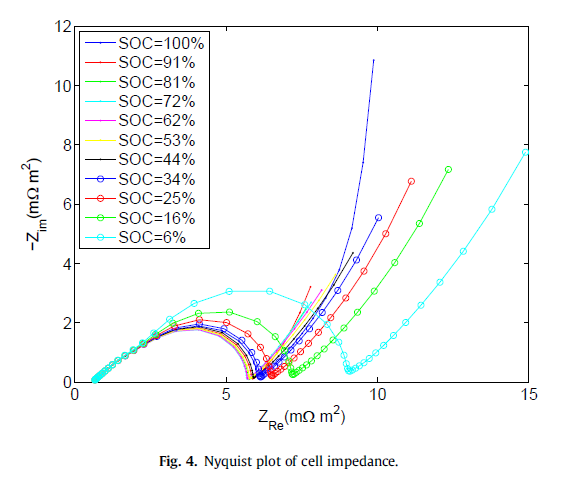
\includegraphics[width=0.7\textwidth]{EIS_Nyquist.png}
	\caption{Diagrama de Nyquist - Espectroscopía Dieléctrica (EIS) de 
	una batería de Li-Ion obtenida por barrido frecuencial.}
	\label{EIS_Nyquist}
    \end{center}
\end{figure}
\FloatBarrier

\subsection{Filtros de Kalman}

Este tipo de filtros toma importancia en sistemas de naturaleza estocástica.
Cuya dinámica es afectada por ruido cuya distribución de probabilidad es
Gaussiana o Normal. Este es un algoritmo recursivo que corrige las estimaciones
mediante la probabilidad conjunta de una o varias mediciones de un fenómeno y su
estimación obtenida por modelos matemáticos generados en base al conocimiento
del sistema.

Dado un sistema lineal cuya dinámica es descripta por las siguientes ecuaciones:

\begin{equation}
    x_{k+1}= Ax_{k} + w_{k}
    \label{KF_equation01}
\end{equation}	

\noindent Donde $\mathrm{x_{k}}$ es el vector de estados en el instante de 
tiempo k, A es la matriz de transición de estados y $\mathrm{w_{k}}$ ruido 
aditivo gaussiano asociado al modelo del proceso con matriz de varianza Q. 
Además podemos expresar el vector de observación o medición $\mathrm{z_{k}}$ 
de los estados $\mathrm{x_{k}}$ como:

\begin{equation}
    z_{k}= Hx_{k} + v_{k}
    \label{KF_equation02}
\end{equation}	

Donde H es la matriz de conexión entre los estados y las observaciones sin
ruido, es decir que mediciones se están tomando y que estado representan. Por
otro lado $v_{k}$ es el ruido aditivo gaussiano asociado a la medición con
matriz de varianza R.

Definiendo la función de costo al error cuadrático medio en la estimación de
$x_k$ 

Definiendo al error como: 

\begin{equation}
    e_{k} = x_k  - \hat{x}_k
    \label{KF_error}
\end{equation}	

De manera que podemos expresar la Matriz de covarianza del error en el instante
k como:

\begin{equation}
    P_{k} = E[e_k.{e_k}^{T}] = E[(x_k-\hat{x}_k).(x_k-\hat{x}_k)^{T}]
    \label{KF_equation03}
\end{equation}	

Podemos expresar $\hat{x}_k$ como: 

\begin{equation}
    \hat{x}_k = \hat{x}^\prime_k + K_k (z_k - H\hat{x}^\prime_k)
    \label{KF_equation04}
\end{equation}	

Donde $K_k$ es la ganancia de Kalman la cual pondera según el criterio de
minimización del error cuadrático medio si $\hat{x}_k$ es próxima a
$\hat{x}^\prime_k$ o al vector $z_k$.

Si reemplazamos $z_k$ en la ecuación \ref{KF_equation04} por la expresión
\ref{KF_equation02} se obtiene la expresión del error de la estimación a priori
$\hat{x}^\prime_k$ detallada a continuación:

\begin{equation}
    \hat{x}_k = \hat{x}^\prime_k + K_k (Hx_{k} + v_{k} - H\hat{x}^\prime_k)
    \label{KF_equation05}
\end{equation}	

Reacomodando los terminos, 

\begin{equation}
    \hat{x}_k = \hat{x}^\prime_k + K_k H (x_{k}  - \hat{x}^\prime_k) + K_kv_{k}
    \label{KF_equation06}
\end{equation}	

Multiplicando por (-1) y luego sumando en ambos miembros de la ecuación
\ref{KF_equation06} el termino $x_k$ 

\begin{equation}
    x_k - \hat{x}_k = x_{k} -\hat{x}^\prime_k - K_k H (x_{k}  - \hat{x}^\prime_k) - K_kv_{k}
    \label{KF_equation08}
\end{equation}	

\begin{equation}
    x_k - \hat{x}_k = (I-K_k H)(x_k - \hat{x}^\prime_k) - K_kv_{k}
    \label{KF_equation09}
\end{equation}	

Reemplazando luego en la ecuación \ref{KF_equation03} la expresión $x_k -
\hat{x}_k$  por el de la ecuación \ref{KF_equation09} obtenemos la expresión de
$P_k$ como función del error de la estimación a priori:

\begin{equation}
    P_k = E[[(I-K_k H)(x_k - \hat{x}^\prime_k) - K_kv_{k}][ (I-K_k H)(x_k - \hat{x}^\prime_k) - K_kv_{k}]^T]
    \label{KF_equation10}
\end{equation}	

\noindent Aplicando propiedades de la transpuesta de una matriz e ignorando 
los terminos relativos a la correlación entre el ruido de la medición y el 
error de la estimación a priori:

\begin{equation}
    P_k = E[[(I-K_k H)(x_k - \hat{x}^\prime_k)(x_k - \hat{x}^\prime_k)^T(I-K_k H)^T + K_k v_{k} v_{k}^T K_k^T 
    \label{KF_equation11}
\end{equation}	

Teniendo en cuenta que la esperanza de una matriz que no es variable aleatoria
es la misma matriz:

\begin{equation}
    P_k = (I-K_k H) E[(x_k - \hat{x}^\prime_k)(x_k - \hat{x}^\prime_k)^T](I-K_k H)^T + K_k E[v_{k} v_{k}^T] K_k^T 
    \label{KF_equation12}
\end{equation}	

\noindent Obteniendose así la expresión de la ecuación de actualización de 
la matriz de covarianza:

\begin{equation}
    P_k = (I-K_k H)P^\prime_k(I-K_k H)^T + K_k R K_k^T 
    \label{KF_equation13}
\end{equation}	

Recordando la forma de la matriz $P_k$ y observando que su traza, es decir, la
sumatoria de todos los elementos de la diagonal principal, es la suma del error
cuadrático medio,de manera que podemos afirmar que minimizando la traza podemos
minimizar el ECM o MSE por su sigla en inglés, \emph{Mean Square Error}.

\begin{equation}
    P_k = 
    \begin{bmatrix}
	e_{1k}e_{1k} & e_{1k}e_{2k} &	\dots  & e_{1k}e_{nk} \\
	e_{2k}e_{1k} & e_{2k}e_{2k} &	\dots  & e_{2k}e_{nk} \\
	\vdots       &   \vdots     &	\ddots & \vdots       \\
	e_{nk}e_{1k} & e_{nk}e_{2k} &	\dots  & e_{nk}e_{nk} \\
    \end{bmatrix}
\end{equation}

De manera que buscamos $K_k$ que cumpla con este requisito, para lo cual haremos
la expansión de la ecuación \ref{KF_equation13}  para obtener luego una
expresión de la traza.

\begin{equation}
    P_k = P^\prime_k - K_k H P^\prime_k - P^\prime_k H^T K^T_k + K_k (H P^\prime_k H^T + R) K^T_k
    \label{KF_equation14}
\end{equation}	

Siendo la expresión de $T[P_k]$

\begin{equation}
    T[P_k] = T[P^\prime_k] - T[K_k H P^\prime_k] - T[P^\prime_k H^T K^T_k] + T[K_k (H P^\prime_k H^T + R) K^T_k]
    \label{KF_equation15}
\end{equation}	

Ya que $P^\prime_k$ es simétrica  y que la traza de una matriz es igual a la
traza de su transpuesta.

\begin{equation}
    P^{\prime T}_k  = P^\prime_k
    \label{KF_equation16}
\end{equation}	

\noindent Podemos escribir

\begin{equation}
    P^\prime_k H^T K^T_k = P^{\prime T}_k H^T K^T_k = (K_k H P^\prime_k )^T
    \label{KF_equation17}
\end{equation}	

\begin{equation}
    T[P^\prime_k H^T K^T_k] = T[K_k H P^\prime_k]
    \label{KF_equation18}
\end{equation}	

Reemplazando \ref{KF_equation18} en \ref{KF_equation15}

\begin{equation}
    T[P_k] = T[P^\prime_k] -2 T[K_k H P^\prime_k] + T[K_k (H P^\prime_k H^T + R) K^T_k]
    \label{KF_equation19}
\end{equation}	

\noindent Para obtener el valor mínimo calculamos la derivada de 
$\mathrm{T[P_k]}$ respecto a $\mathrm{K_k}$

\begin{equation}
    \frac{dT[P_k]}{dK_k} = -2 (H P^\prime_k)^T + 2K_k (H P^\prime_k H^T + R)
    \label{KF_equation20}
\end{equation}	

\noindent Luego igualando la ecuación \ref{KF_equation20} a 0 y despejando 
obtenemos la expresión de la Ganancia de Kalman ($\mathrm{K_k}$):

\begin{equation}
    K_k = (H P^\prime_k)^T (H P^\prime_k H^T + R)^{-1} 
    \label{KF_equation21}
\end{equation}	

\noindent Definiendo a $\mathrm{S_k}$ como:

\begin{equation}
    S_k = (H P^\prime_k H^T + R)
    \label{KF_equation22}
\end{equation}	

\noindent La ecuación \ref{KF_equation21} queda:

\begin{equation}
    K_k = (H P^\prime_k)^T S_k^{-1} 
    \label{K_Gain}
\end{equation}	

\noindent Reemplazando la expresión de $\mathrm{K_k}$ obtenido, en la 
ecuación  \ref{KF_equation14}, se cancela el tercer término con el cuarto 
término y queda:

\begin{align}
    P_k  &= P^\prime_k + P^\prime_k H^T (H P^\prime_k H^T + R)^{-1} H P^\prime_k \nonumber \\
    P_k  &= P^\prime_k - K_k H P^\prime_k \nonumber\\
    P_k  &= (I - K_k H) P^\prime_k	
    \label{KF_equation23}	
\end{align}

\noindent La proyección del vector de estados $\mathrm{x_k}$ en el instante 
$\mathrm{k+1}$ se obtiene como:

\begin{equation}
    \hat{x}^\prime_{k+1} = A \hat{x}_k 
    \label{x_k_projection}
\end{equation}	

\noindent Para luego proyectar la matriz de covarianza de error
$\mathrm{P_k}$ en el instante $\mathrm{k+1}$.

\noindent Haciendo uso de la ecuación \ref{KF_equation03} y extendiéndola 
para $\mathrm{e^\prime_{k+1}}$:

\begin{equation}
    P_{k+1} = E[e_{k+1}.e_{k+1}^{T}] = E[(A e_k-w_k).(A  e_k-w_k)^{T}]
    \label{projection_p_k_aux}
\end{equation}	

\noindent Cabe destacar que el ruido del proceso $\mathrm{w_k}$ no tiene 
correlación alguna respecto a $\mathrm{e_k}$ ya que el primero es el ruido 
presente entre k y k+1 y $\mathrm{e_k}$ es el error resultante de todos los 
calculos previos hasta el instante k.

\begin{equation}
    P^\prime_{k+1} = E[A e_{k}.e_{k}^{T}A^{T}]+ E[w_k w_k^{T}]= A P_k A^{T} + Q
    \label{projection_p_k}
\end{equation}	

\subsubsection{Filtro de Kalman: resumen}

Como dijimos los filtros de Kalman son algoritmos recursivos, los mismos se
componen por las siguientes ecuaciones descriptas anteriormente:

\begin{table}[h!]
    \centering
    \begin{tabular}{|c|c|}
	\hline
	\rule{0pt}{4ex}	Ganancia de Kalman 							& $K_k = (H P^\prime_k)^T S_k^{-1}$  \\ \hline
	\rule{0pt}{4ex}	Actualización de la estimación			    &  $\hat{x}_k = \hat{x}^\prime_k + K_k (z_k - H\hat{x}^\prime_k)$\\ \hline
	\rule{0pt}{4ex}	Actualización de la matriz de covarianza    & $P_k = (I - K_k H) P^\prime_k$ \\ \hline
	\multirow{2}{*}{Proyeccion en k+1}        		  			& \rule{0pt}{4ex} $\hat{x}^\prime_{k+1} = A \hat{x}_k$ \\ \cline{2-2}
	& \rule{0pt}{4ex} $P^\prime_{k+1} = A P_k A^{T} + Q$ \\ \hline
    \end{tabular}
    \label{Ecuaciones_Kalman}
\end{table}

Una manera intuitiva de pensar los filtro de Kalman es de la siguiente.
Supongamos que tenemos la medición antes definida como $z_k$ y corriendo en
paralelo tenemos un modelo matemático calculando el estado actual o vector de
estados actual de nuestro sistema el cual notaremos como $\hat{x}^\prime_k$ y
llamaremos estimación a priori de $x_{t}$.

Ambos valores son afectados por ruido asociado, de manera que podemos ponderar
ambas de manera de obtener una medición más certera.

Como se observa en la Fig. \ref{KF_Integration_concept} en base a las
distribuciones de $z_k$ y $\hat{x}^\prime_k$ obtenemos una nueva $\hat{x}_k$ la
cual tiene una menor varianza.

\begin{figure}[h!]
    \begin{center}
	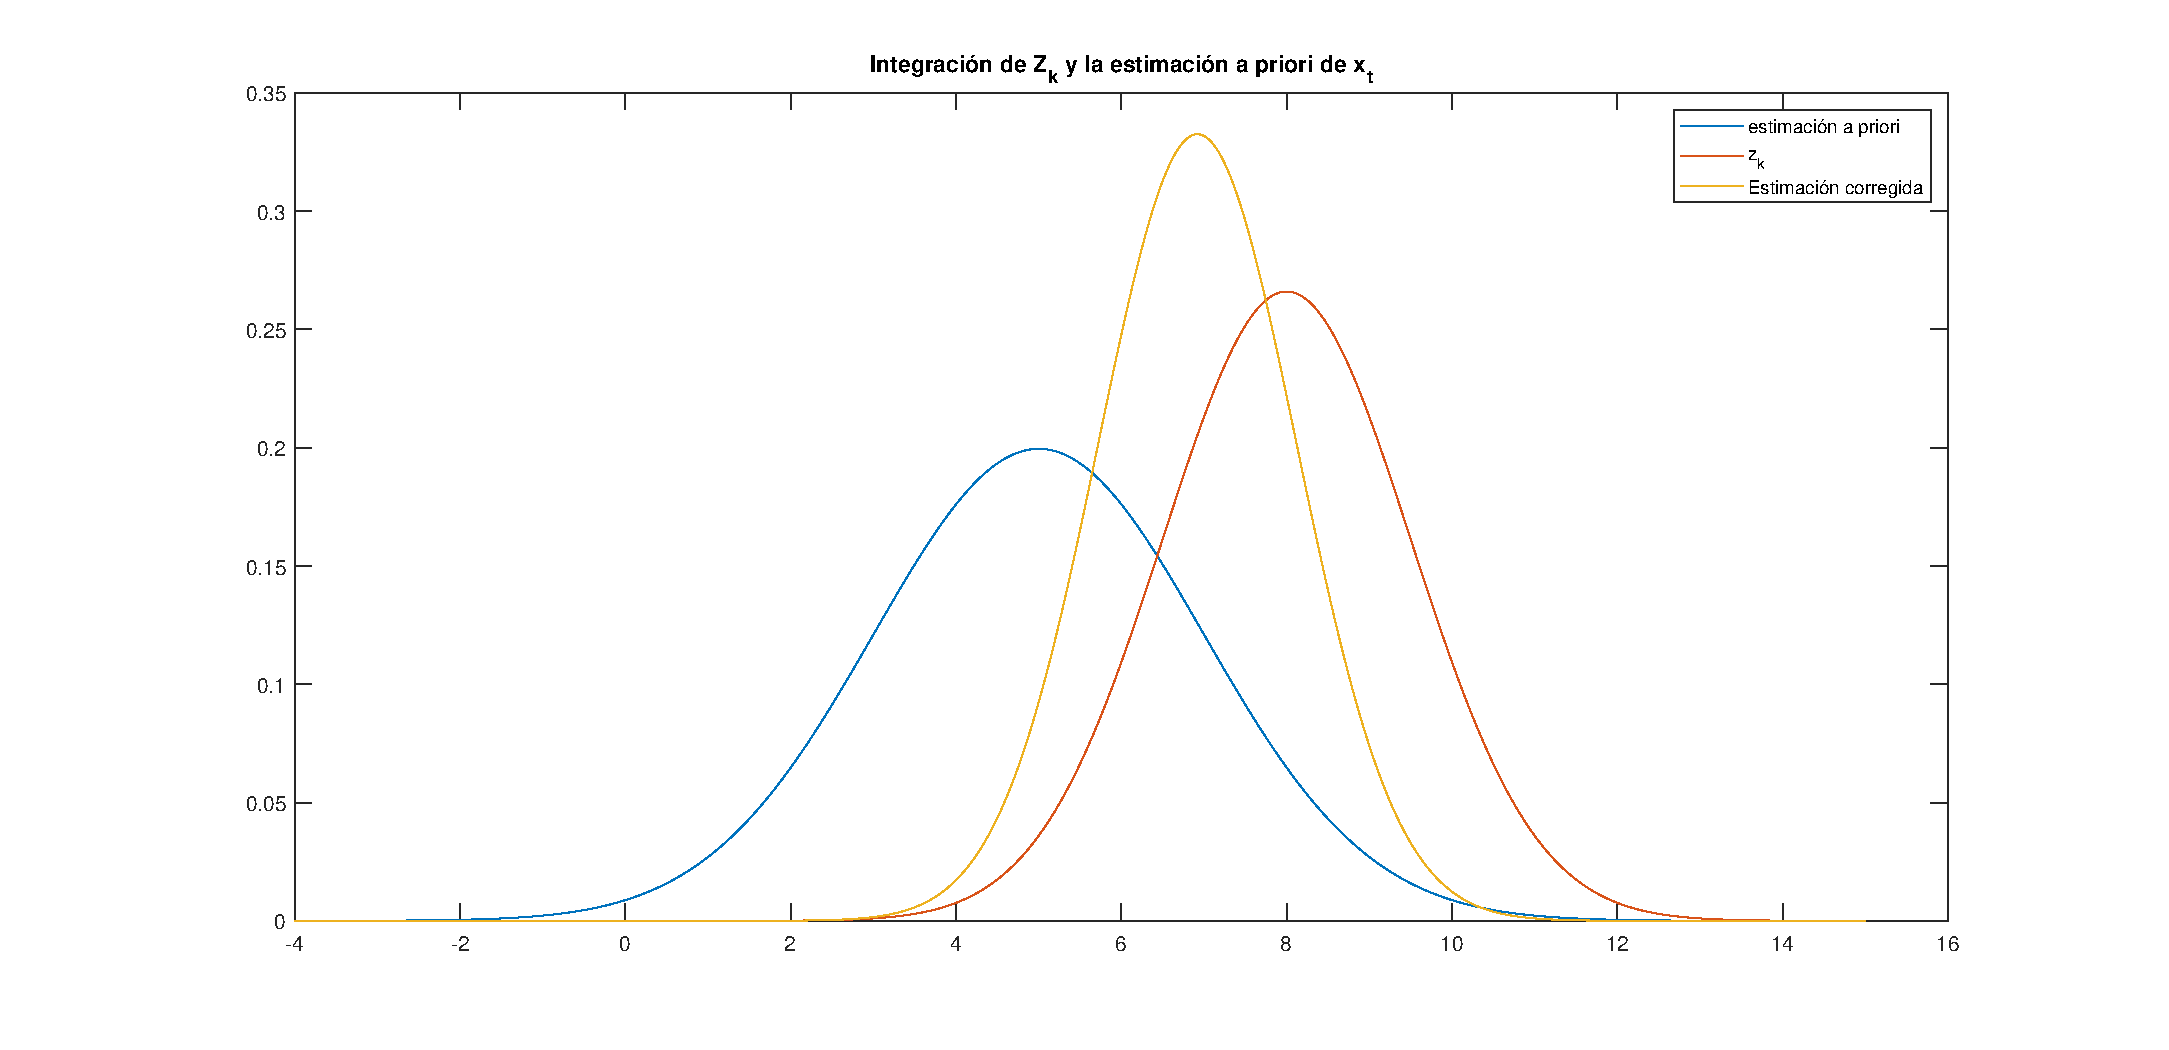
\includegraphics[width=1\textwidth]{KF_Integration_concept.eps}
	\caption{Gráfico ilustrativo de la estimación de $x_{t}$ mediante $z_k$ y
	$\hat{x}^\prime_k$ .}
	\label{KF_Integration_concept}
    \end{center}
\end{figure}
\FloatBarrier

\subsection{Simulaciones}

\subsubsection{Simulación Filtro de Kalman}

Para la implementación de este filtro es necesario obtener un modelo en espacio
de estados de la batería de la forma :

\begin{align}
    \dot{x}(t) = Ax+Bu	\nonumber\\
    y(t)=Cx+Du
    \label{SS_Model_generic}	
\end{align}

Para tal fin tomamos como referencia un modelo eléctrico con 2 elementes RC en
serie, también conocido como modelo de Randles de segundo orden, representado en
la figura \ref{Randles_2do}, ya que este módelo tiene amplia aceptación debido a
que ofrece un grado de ajuste alto sin resultar en un excesivo costo
computacional en comparación con modelos electroquímicos de la batería.

\begin{figure}[h!]
    \begin{center}
	\begin{minipage}[c]{0.95\textwidth}
	    \centering
	    \ctikzset{bipoles/length=1.0cm}
	    \ctikzset{bipoles/resistor/height=.3}

	    \begin{circuitikz}[american]

		\draw (0,0) to[R=$R_0$] (3,0) -- (3,-0.5) to[R=$R_1$] (6,-0.5) -- (6,0);
		\draw (3,0) -- (3,0.5) to[C=$C_1$,v=$ $] (6,0.5) -- (6,0);
		\draw (6,0) to[short,-*] (6.5,0) -- (7,0) -- (7,0.5) to[C=$C_2$,v=$ $] (10,0.5) to[short,-o] (10,0);
		\draw (7,0) -- (7,-0.5) to[R=$R_2$] (10,-0.5) -- (10,0) to[short,f=$i$] (11.5,0);
		\draw  (0,0) to[battery2=$OCV(SOC)$] (0,-3) -- (11.5,-3); 
		\draw  (11.5,0) to [open,v=$v$,invert] (11.5,-3);
		\draw (8.5,1.75) node[anchor=north]{$V_{C2}$};
		\draw (4.5,1.75) node[anchor=north]{$V_{C1}$};
	    \end{circuitikz}
	\end{minipage}
    \end{center}
    \caption{Circuito de Randles de Segundo Orden.}
    \label{Randles_2do}
\end{figure}
\FloatBarrier

\noindent La fuente de tensión controlada $OCV(SoC)$ es linealizada para 
obtener un modelo lineal de la batería e ignoramos el hecho de la histéresis 
respecto a la carga y a la descarga.

Obteniendo una ecuación lineal de la forma \ref{SOC_linearized}, cuyos
parametros fueron obtenidos mediante la función \emph{polyfit} de matlab como se
muetra en la figura \ref{SOC_vs_OCV}.

\begin{equation}
    OCV = SOC \times K_e + OCV_0
    \label{SOC_linearized}
\end{equation}

\begin{figure}[h!]
    \begin{center}
	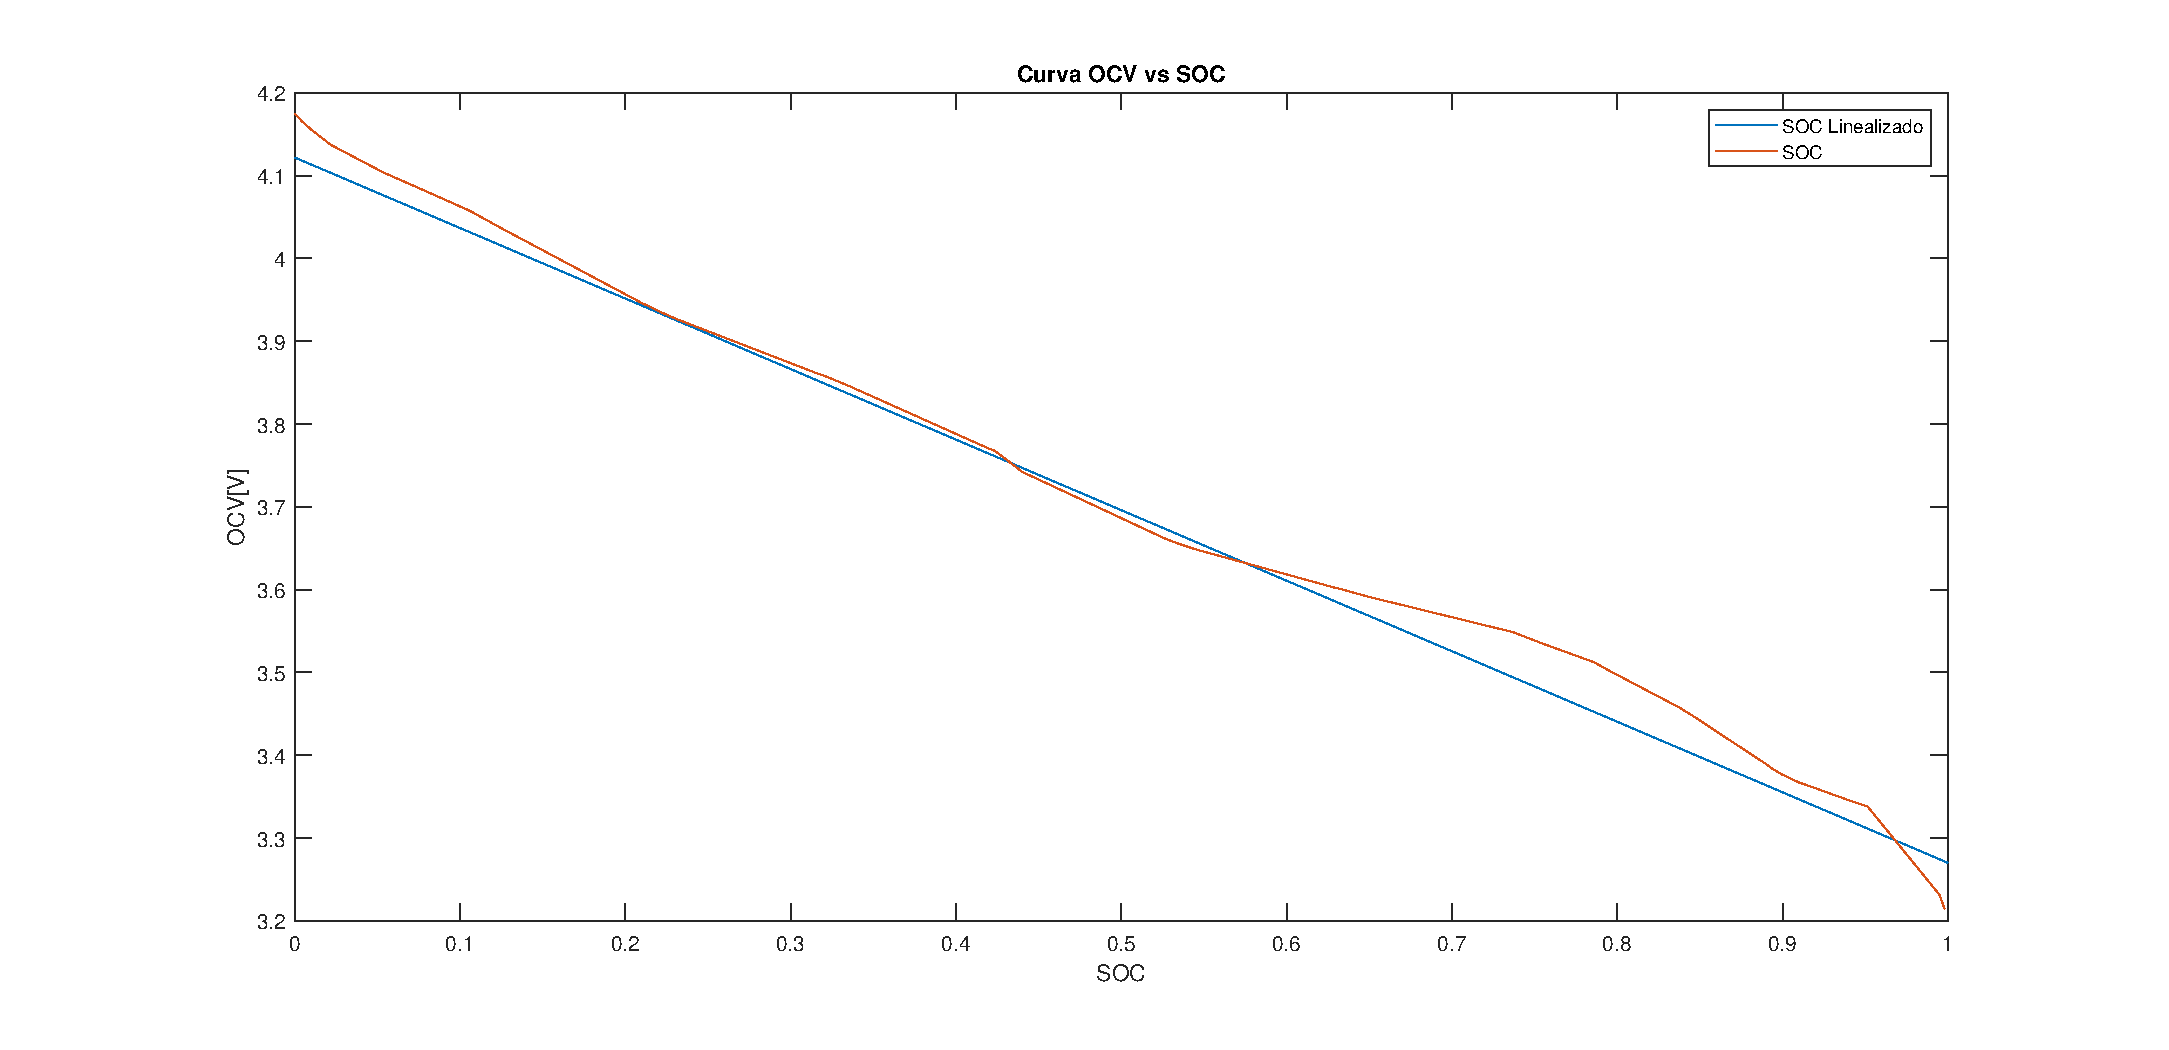
\includegraphics[width=1\textwidth]{SOC_vs_OCV.eps}
	\caption{Curva de SOC vs OCV con su correspondiente linealización }
	\label{SOC_vs_OCV}
    \end{center}
\end{figure}
\FloatBarrier

Nuestro modelo eléctrico tiene 2 grados de libertad y se agrega una 3° variable
de estado que es el estado de carga de la batería. Luego tomando la expresión
diferencial de la ecuación \ref{SOC_Coulomb_C}, seleccionando arbitrariamente
las tensiones en $C_1$ y $C_2$, y tomando como entrada del sistema la corriente
de la batería y como salida la tensión en bornes de la misma obtenemos el
siguiente conjunto de ecuaciones.

\begin{equation}
    \begin{array}{llcllcl}
	\dot{x} & = & \begin{bmatrix}
	    -\frac{1}{R_1 C_1} &            0       & 0 \\
	    0                  & -\frac{1}{R_2 C_2} & 0 \\
	    0                  &            0       & 0 \\
	\end{bmatrix} & x & + &     \begin{bmatrix}
	    -\frac{1}{R_1 C_1} \\
	    -\frac{1}{R_2 C_2}  \\
	    -\frac{1}{3600 S_{C,a}}\\
	\end{bmatrix} & i \\
	\\
	y & = & \begin{bmatrix}
	    -1-1-K_e 
	\end{bmatrix} & x & + & \begin{bmatrix}
	    R_0
	\end{bmatrix} & i \\
    \end{array}
\end{equation}

Donde $S_{C,a}$ es la Capacidad Nominal en Ah de la batería. 

Para hacer un ajuste de parámetros de las baterías se utilizó un dataset
provisto por la universidad de Winsconsin-Madison por el Dr. Phillip Kollmeyer
\cite{Kollmeyer2018}. si bien todos los parámetros son dependientes del estado
de carga, seleccionamos los correspondientes al 90\%, ya que las variaciones mas
fuertes de los mismos se dan al entre el 0-10\% y en valores cercanos al 100\%

\begin{figure}[h!]
    \begin{center}
	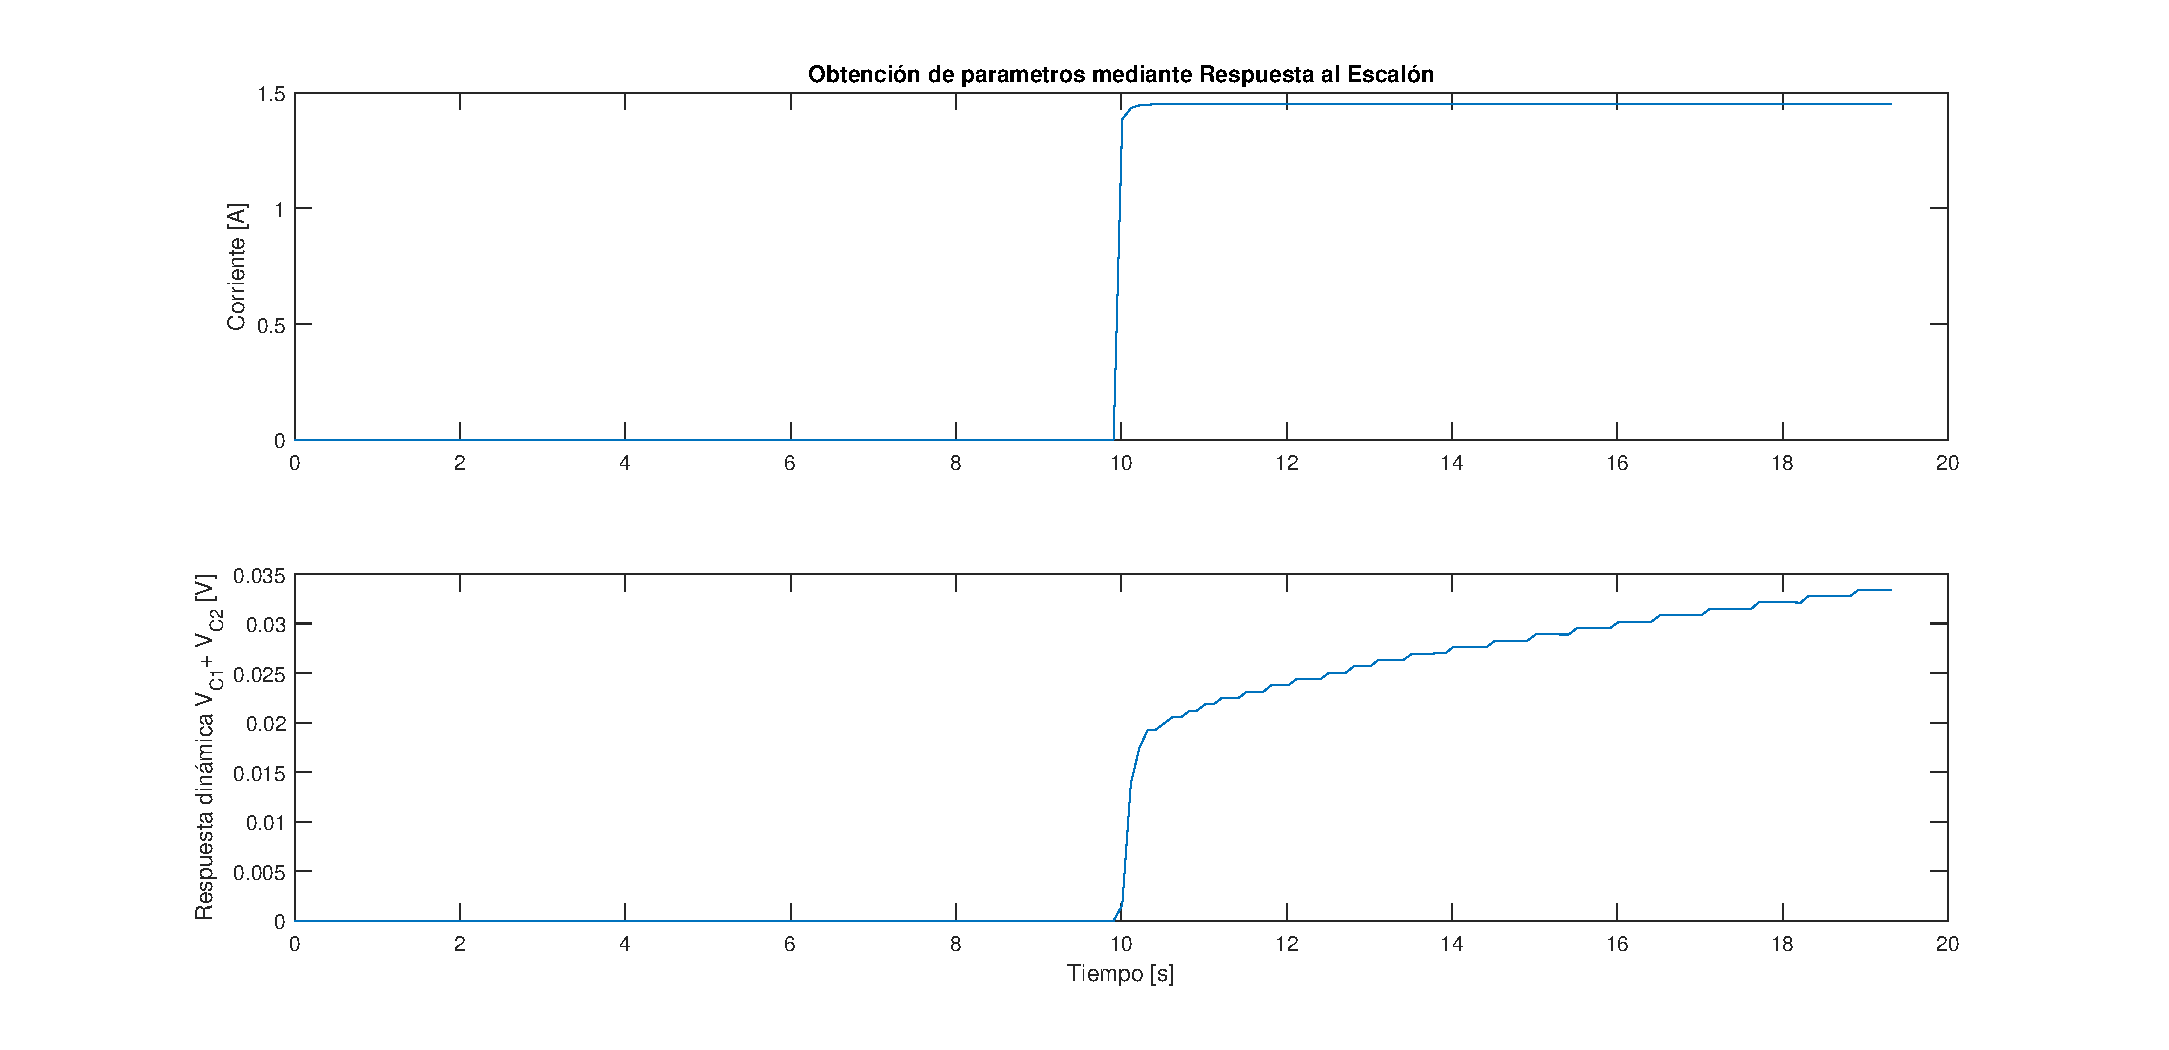
\includegraphics[width=0.85\textwidth]{rta_escalon.eps}
	\caption{Estudio de la Rta al escalón para estimación de parámetros}
	\label{rta_escalon}
    \end{center}
\end{figure}
\FloatBarrier

También se necesita proporcionar valores de Varianza del modelo, ruido al que
están sometidas las variables medibles, el estado inicial estimado y la varianza
de esta estimación estas son denominadas Q,R,$x_0$ y $P_0$ respectivamente.

\noindent Partiendo de la base que nuestro sistema debe ser robusto ante la mala
estimación inicial del estado de carga vamos a proponer un vector de estimación
de estado inicial con un SoC con un error de 80\%.

\begin{equation}
    \begin{array}{llll}
	P_0 & = & \begin{bmatrix}
	    1 & 0 & 0 \\
	    0 & 1 & 0 \\
	    0 & 0 & 1 \\
	\end{bmatrix} 
    \end{array} \nonumber
\end{equation}

\noindent El ciclo de la bateria esseleccionado comienza con la batería cargada
al 100\%, por lo que un error del 80\% se corresponde con 0.2 en el estado de
carga relativo.

\begin{equation}
    \begin{array}{llll}
	x_0 & = & \begin{bmatrix}
	    0 \\
	    0 \\
	    0.2 \\
	\end{bmatrix} 
    \end{array} \nonumber
\end{equation}

\noindent El error en nuestra observación es del orden de los milivoltios
(mV) calculado en base a la resolución del sensor.

\begin{equation}
    R = 0.01  \nonumber
\end{equation}

\noindent El error en nuestro modelo se estima bajo ya que los dataset nos 
proveen una buena fuente de información obtenida en base a ensayos de 
laboratorio

\begin{equation}
    \begin{array}{llll}
	Q & = & \begin{bmatrix}
	    1\cdot10^{-6} & 0 & 0 \\
	    0 & 1\cdot10^{-6} & 0 \\
	    0 & 0 & 1\cdot10^{-6} \\
	\end{bmatrix} 
    \end{array} \nonumber
\end{equation}

Por último se volcaron estos parámetros en un bloque de la librería \emph{System
Identification Toolbox} que corre el algoritmo del filtor de Kalman. Además se
simuló en paralelo el circuito eléctrico equivalente, como se observa en la
Figura \ref{simulink_diagram}.

\begin{figure}[h!]
    \begin{center}
	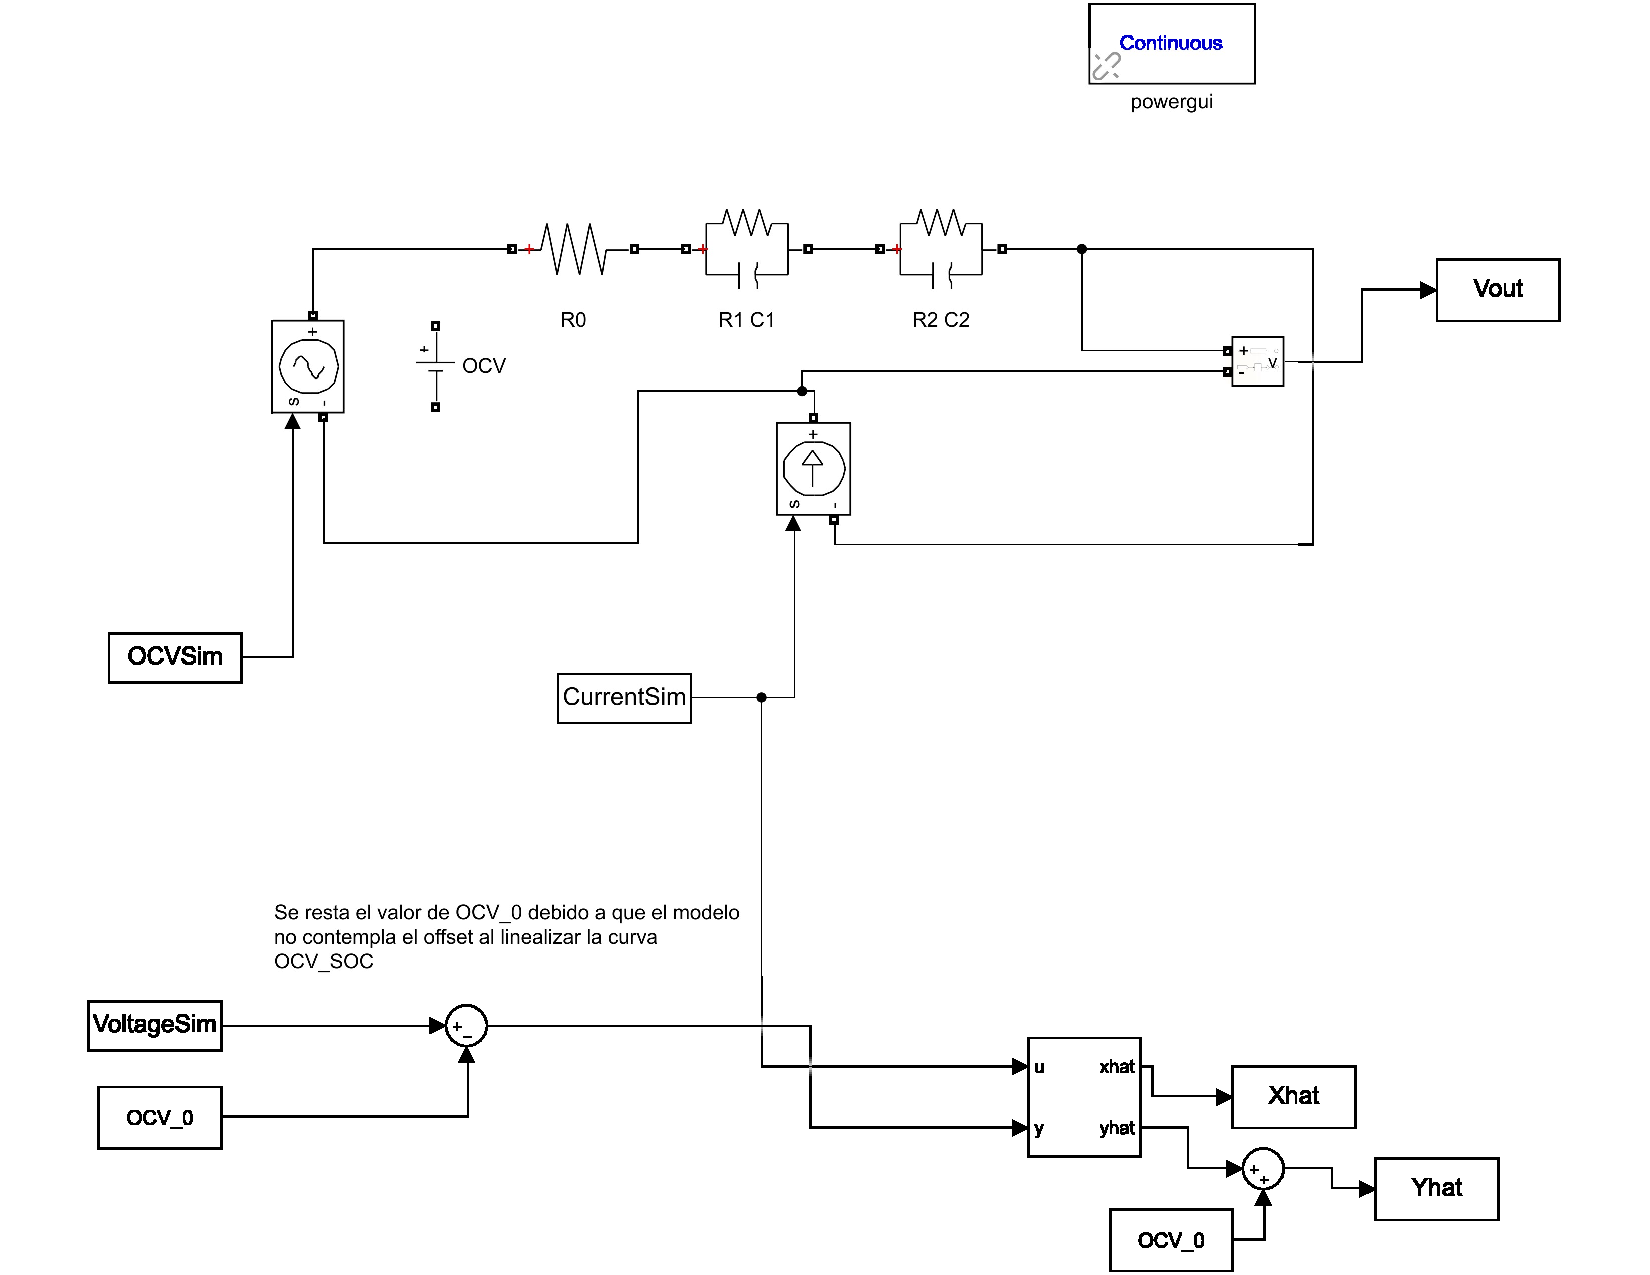
\includegraphics[width=0.95\textwidth]{simulink.pdf}
	\caption{Diagrama de Simulink utilizado para simular el Filtro de Kalman}
	\label{simulink_diagram}
    \end{center}
\end{figure}

Los resultados de la simulación se muestran a continuación en las Figuras
\ref{Tension_sim} y \ref{Tension_sim_zoom} correspondientes a la tensión en
bornes de la batería y  a las Figuras \ref{Drive_Cycle_1_SOC_sim} y
\ref{error_SOC_Sim}, las cuales corresponden al SOC simulado y a un contraste
del error tomando como valor verdadero el SOC provisto por el dataset.

\begin{figure}[h!]
    \begin{center}
	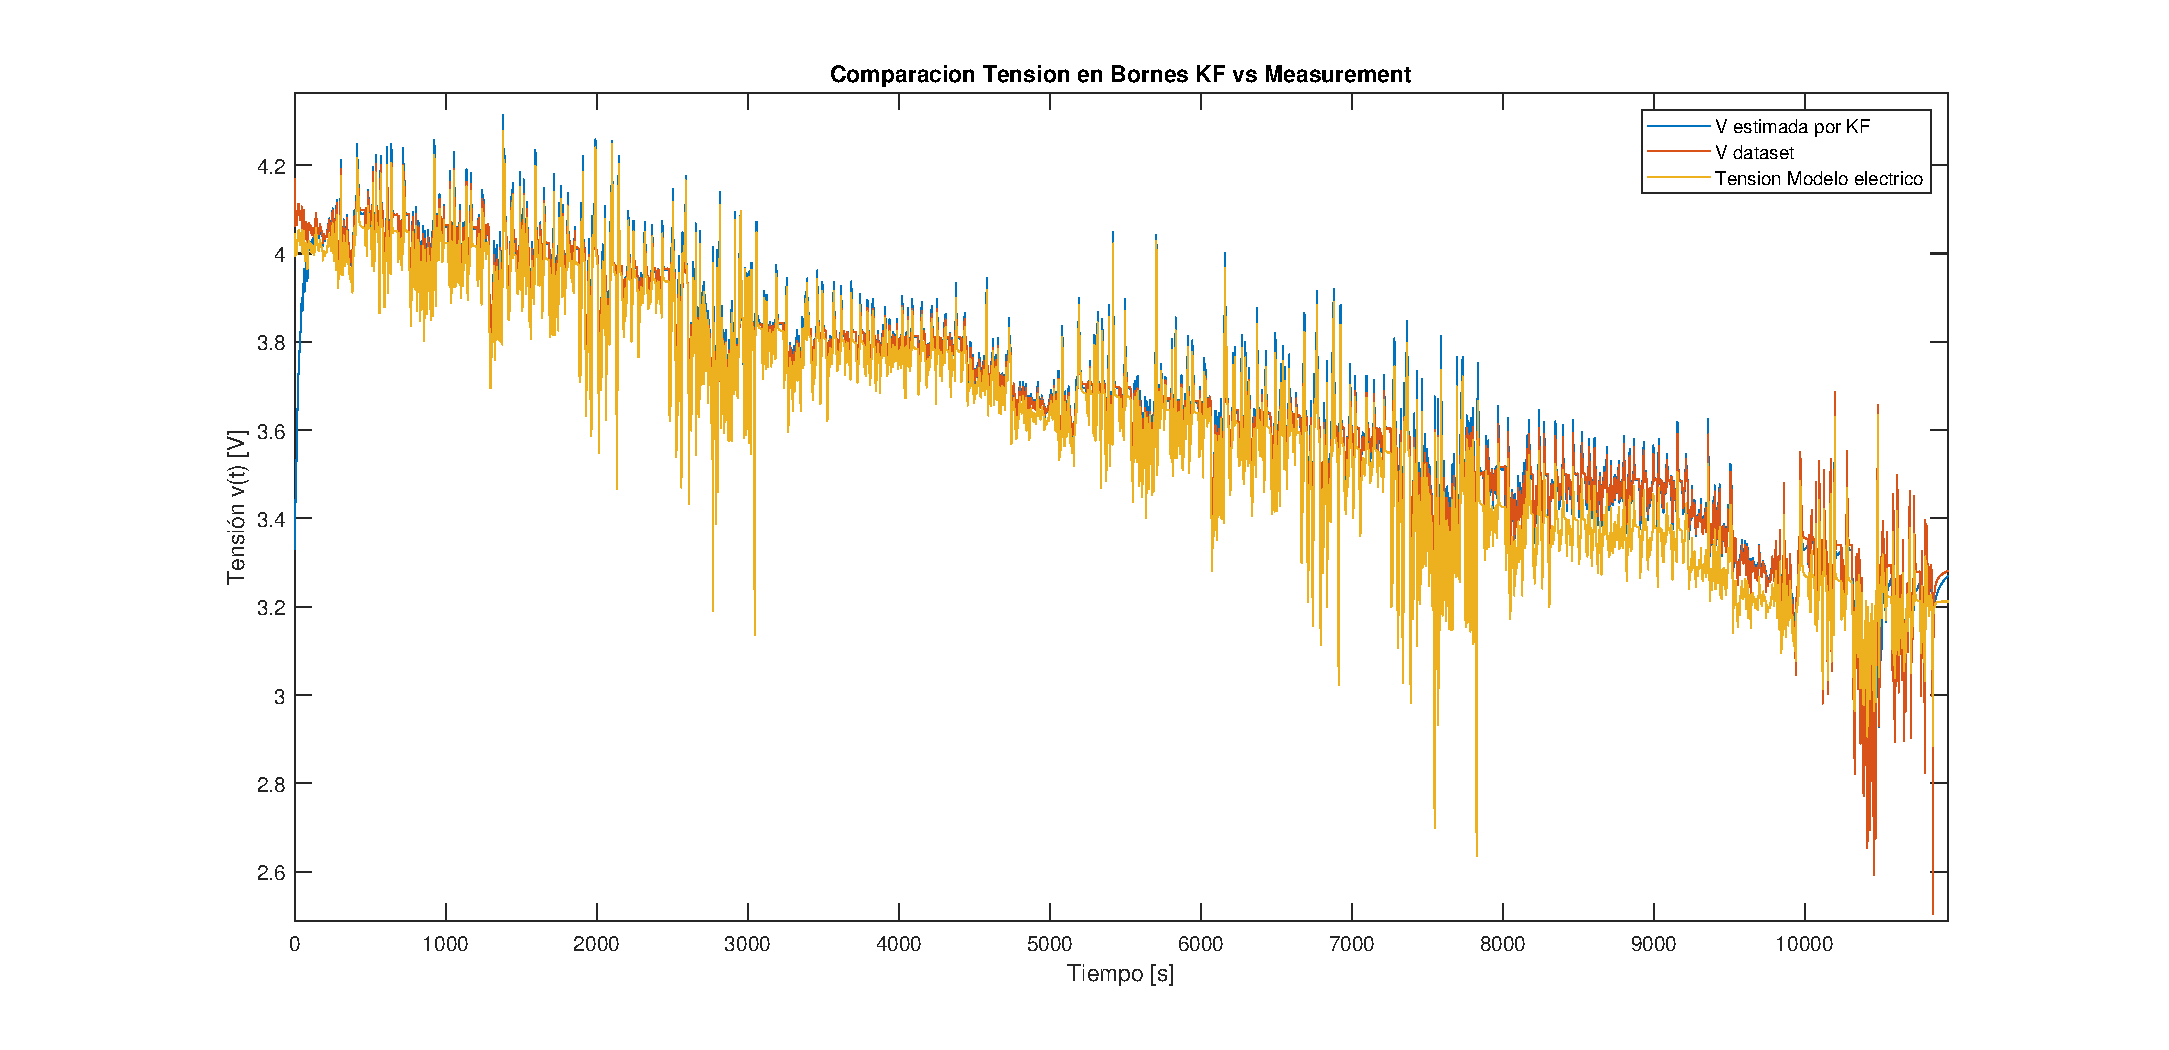
\includegraphics[width=1\textwidth]{Tension_Sim.eps}
	\caption{Resultado de la Simulación de la tensión en bornes de la 
	batería sometida a condiciones de ciclo de manejo}
	\label{Tension_sim}
    \end{center}
\end{figure}

\begin{figure}[h!]
    \begin{center}
	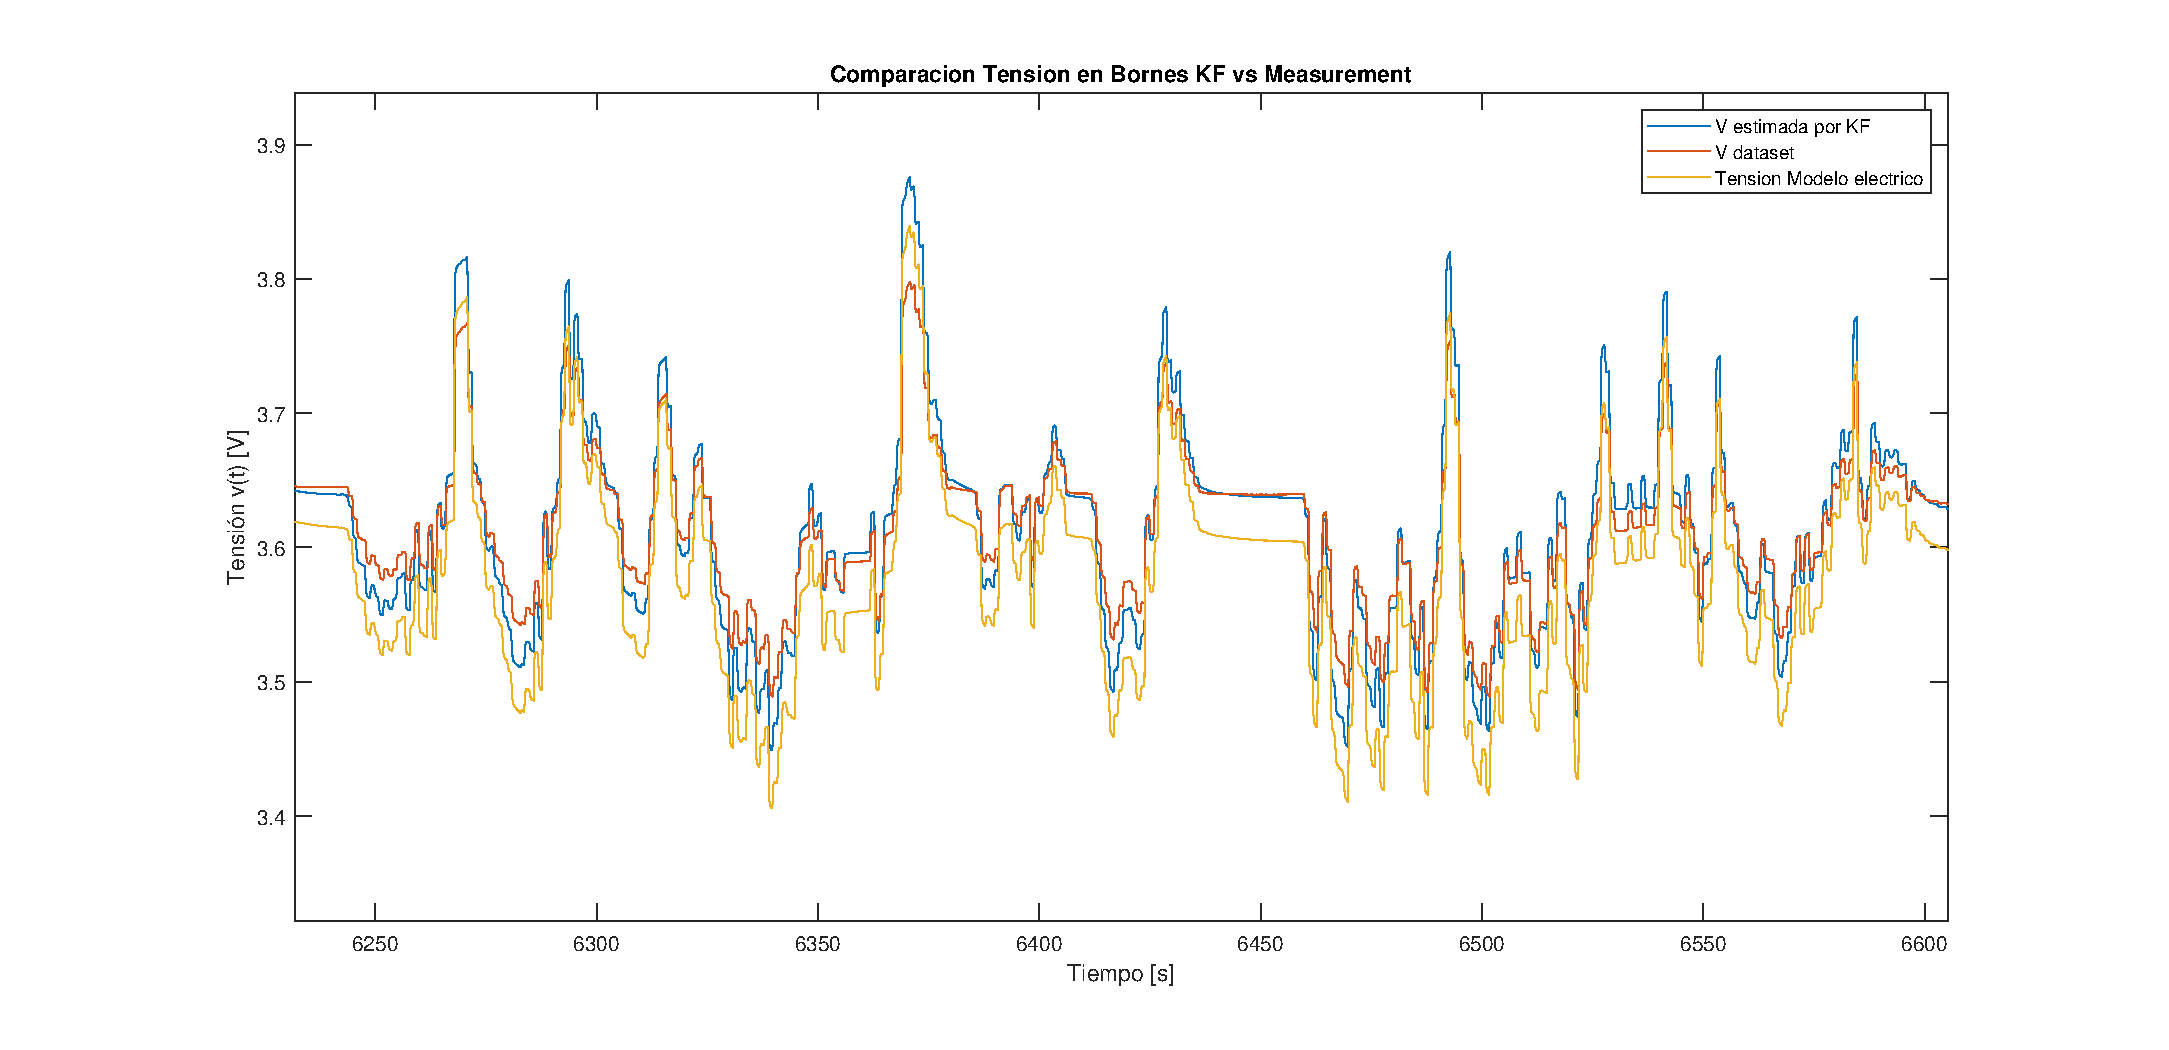
\includegraphics[width=0.95\textwidth]{Tension_Sim_zoom.eps}
	\caption{Detalle de la Simulación de la tensión en bornes de la batería
	sometida a condiciones de ciclo de manejo}
	\label{Tension_sim_zoom}
    \end{center}
\end{figure}

Si se presta especial atención el error se mantiene en una cota del 6 \% hasta
que se dispara en la región de SOC menor al 15\% donde el sistema se vuelve
fuertemente alineal y nuestro modelo pierde validéz. Por otro lado cumple
satisfactoriamente con la corrección del SOC inicial ya que estaba seteado en 20
\% y el Filtro corrige rapidamente a un valor aproximado de 100 \%. 

\begin{figure}[h!]
    \begin{center}
	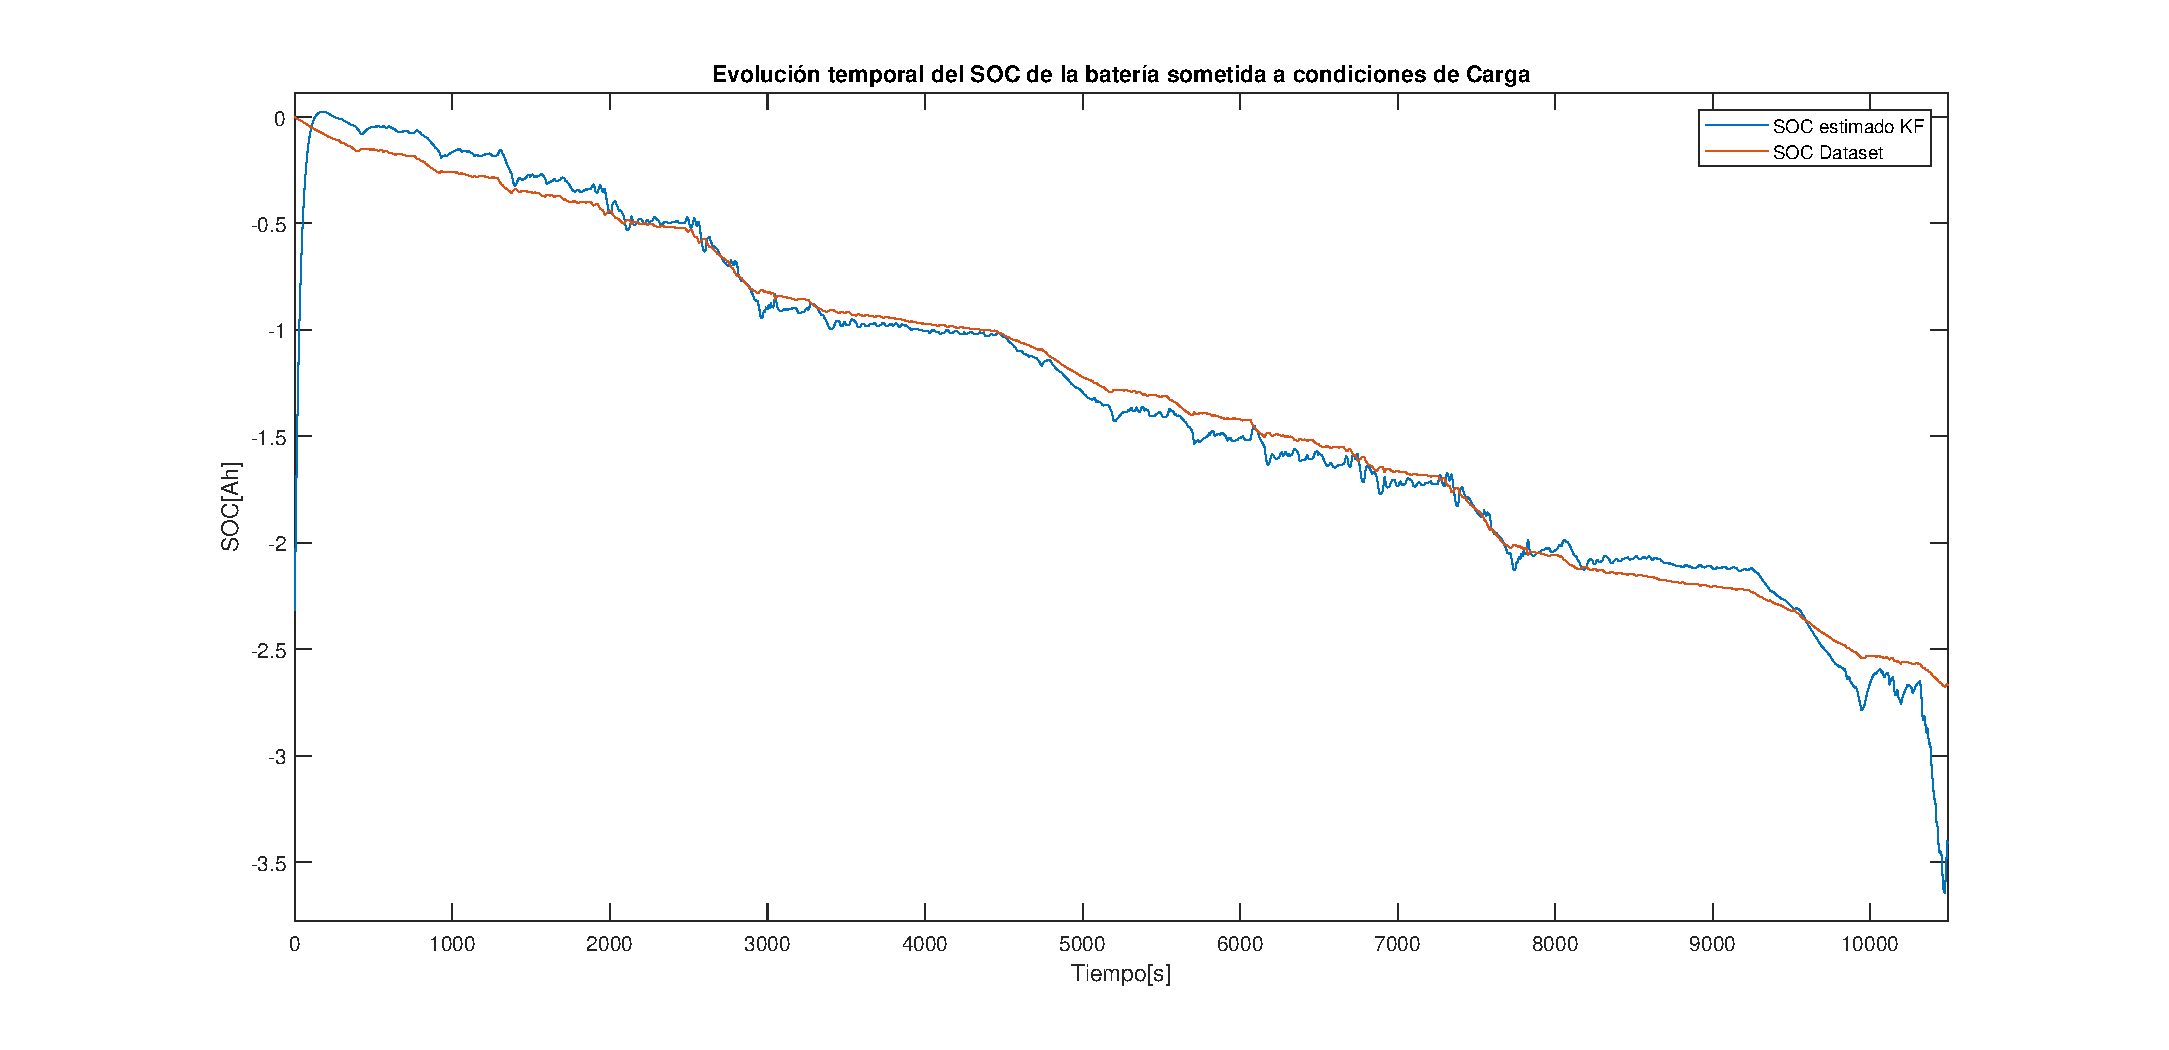
\includegraphics[width=0.95\textwidth]{Drive_Cycle_1_sim.eps}
	\caption{Resultados de la Simulación del sistema sometido a condiciones de
	ciclo de manejo}
	\label{Drive_Cycle_1_SOC_sim}
    \end{center}
\end{figure}

\begin{figure}[h!]
    \begin{center}
	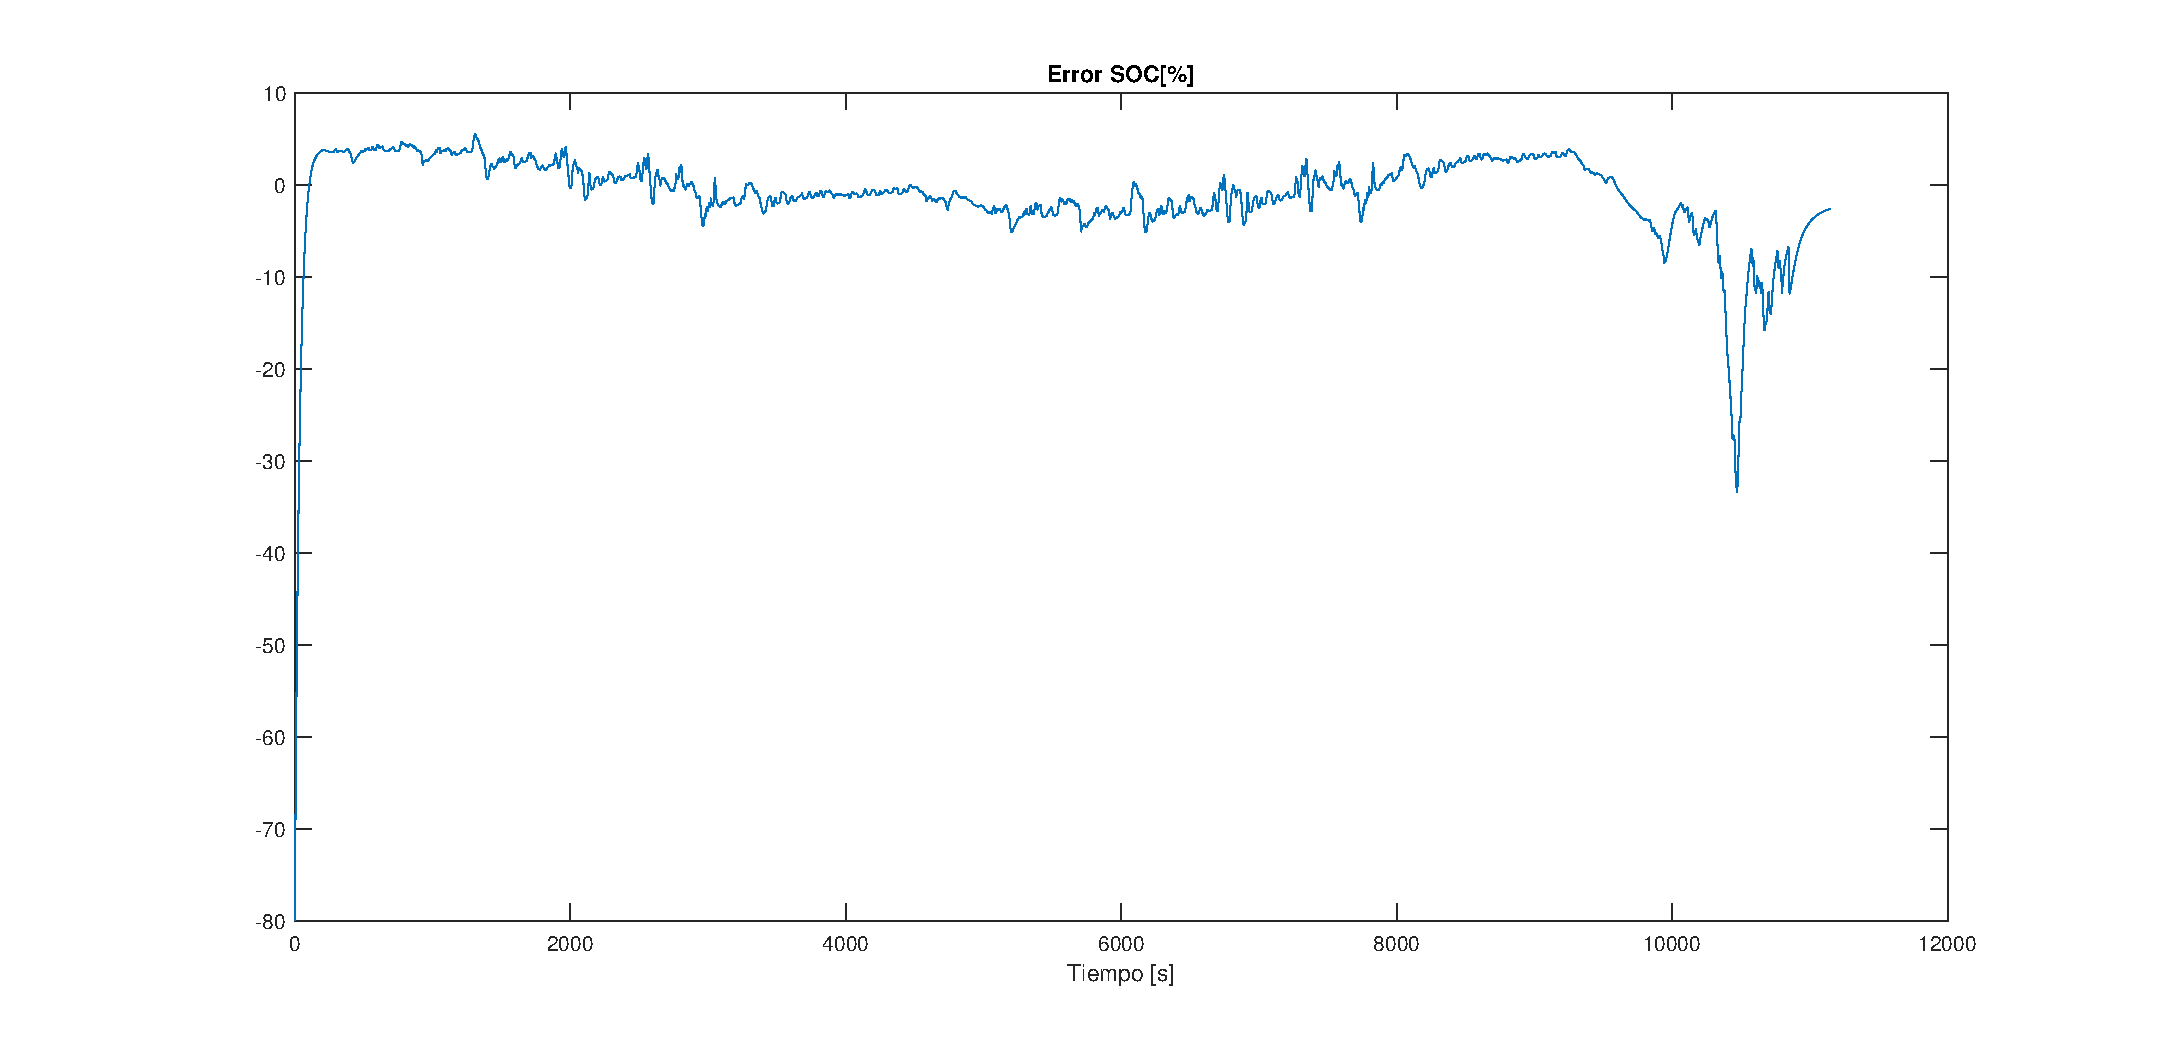
\includegraphics[width=0.95\textwidth]{soc_error_porc.eps}
	\caption{Resultados de Simulación del SOC de una batería sometida a
	condiciones de ciclo de manejo}
	\label{error_SOC_Sim}
    \end{center}
\end{figure}
\FloatBarrier

\subsection{Técnica de Carga} 
\subsubsection{Corriente Constante CC - Voltaje Constante CV}

El proceso de carga de una \acrfull{Ion-Li} no es trivial. Aplicar una tensión
constante en  bornes, como podríamos proceder con baterias de plomo ácido, no es
el procedimiento más adecuado en este caso. En aras de optimizar la autonomía y
la vida útil del pack de baterías el proceso de carga debe responder a
lineamientos particulares deacuerdo a las carácterísticas constructivas de las
celdas que lo componen.

El peril de carga que se ajusta a las celdas de \acrshort{Ion-Li}, como se
observa en la figura \ref{fig:char_prof}, es el perfil \acrfull{CC} -
\acrfull{CV}. Este consiste en tres fases, una primera etapa de
acondicionamiento o pre carga donde se inyecta a la batería una corriente
constante pequeña de magnitud equivalente a la corriente de fin de carga. Una
fase de carga rápida a corriente constante \acrshort{CC} y una tercer y última
fase de carga a tensión constante \acrshort{CV}.

\begin{figure}[h!] \centering
    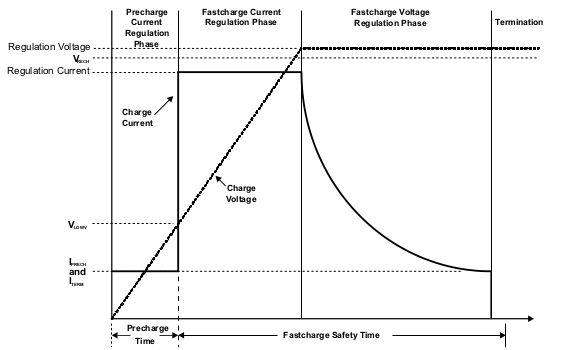
\includegraphics[width=0.8\textwidth]{bat_char/char_profile.png}
    \caption{Perfil de carga típico de una batería de Ion-Litio}
\label{fig:char_prof} \end{figure} \FloatBarrier

El proceso de pre carga o pre-acondicionamiento proporciona a las celdas la
capacidad de recuperar su capa de pasivación, la cual puede haberse visto
afectada o disuelta tras largos periodos de almacenamiento en estados de
descarga profunda. A su vez permite introducir las celdas en la zona de
operación segura en caso de que se encuente prufundamente descargadas.  Es
importante limitar el proceso de acondicionamiento en tiempo para prevenir pre
cargar indefinidamente una celda que se encuentre agotada. Si tras un periodo
completo de acondicionamiendo la celda no alcanza el voltaje mínimo necesario
puede considerarse que la misma alcanzó el final de su vida útil.

El voltaje umbral de inicio de carga rápida depende de la celda misma y en el
caso de las baterías \acrshort{Ion-Li} se ubica generalmente entre los $2.5V$ y
$3.0V$.  Una vez que la celda supera su voltaje umbral mínimo el cargador debeŕa
entra en la zona de carga rápida a corriente constante \acrshort{CC}. La fase de
carga rápida permite a la batería transformar la enería eléctria entregada en
energía electroquímica dentro de la batería en el menor tiempo posible. La
magnitud de la corriente de carga rápida depende de la celda y es limitada
generalmente entre $0.5C$ y $1C$ para prevenir el calentamiento del pack y su
degradación prematura. El pack de batería admitrá carga rápida a corriente
constante hasta alcanzar el voltaje límite de regulación. 

En esta tercer y última fase la corriente drenada del pack decae
exponencialmente hasta alcanzar la magnitud de fin de carga, situación que nos
indica que el ciclo se completo exitosamente. La corriente de terminación de
carga ronda entre $5\%$ y $10 \%$ de la corriente de carga rápida. Cabe aclarar
que en esta instancia del proceso de carga la corriente decae naturalmente dado
que es la contante de voltaje de terminales la magnitud controlada por el
cargador.  

Es importante remarcar que durante todo el proceso de carga, pero
fundamentalmente durante la fase de carga rápida a corriente constante, es de
vital importancia monitorear la temperatura de las celdas evitando que las
mismas se aparten de la zona de operación segura. Si bien el proceso de carga
implica intrínsicamente una elevación de la temperatura de la celda, etre otras
causas debido a su resistencia interna.

El tiempo total de carga es una variable determinante a la hora de implementar
un cargador de batería que extienda al máximo la vida útil y los ciclos de carga
de un pack de baterías y de sus celdas. Es la magnitud de corriente de carga
rápida la variable determinante del tiempo final de carga. Por ejemplo, para una
carga rápida a 1C, la bateria alcanzará, durante la fasé de \acrshort{CC}, el
$70\%$ de su capacidad total en el $30\%$ del tiempo de carga mientras que
tardará el $70\%$ del tiempo total de carga para acumular el $30\%$ restante de
su capacidad durante la fase \acrshort{CV}. 

La existencia de una resistencia interna en serie en las celdas no ideales
implica que a mayor corriente de carga rápida a CC se alcance más rápido la
tensión de umbral de paso a la fase de tensión constante CV acortando el tiempo
de CC pero extendiendo el tiempo de CV. Podemos inferir entonces que a menor
resistencia interna menor tiempo de carga. Y que aumentar la corriente a CC
tambien reducirá el tiempo de carga.  Sin embargo, se desaconseja completamente
implementar regímenes de carga rápida que superen 1C por el impacto en el número
de ciclos de vida útil de las celdas del pack de batería. La figura
\ref{fig:C_vs_Cycle_I} muestra como a medida que aumentamos el régimen de carga
de una celda la vida útil de la misma, medido en ciclos de carga, disminuye
significativamente.

\begin{figure}[h!] \centering
    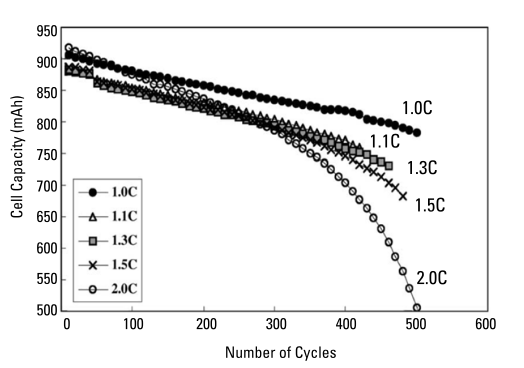
\includegraphics[width=0.6\textwidth]{bat_char/C_vs_Cycle_I.png}
    \caption{Relación Corriente de carga vs Ciclos de vidaútil de una celda de
    Ion-Litio con un cátodo de $LiCoO_2$} \label{fig:C_vs_Cycle_I} 
\end{figure}
\FloatBarrier

A mayores tasas de corriente, mayor cantidad de iones de litio se depositan
sobre el ánodo conviritiendose en litio metálico al librerar sus electrónes
disponibles.  El litio metálico es sumamente reactivo con el electrolito
resultando en una pérdida permanente de \acrshort{Ion-Li}, el elemento
almacendor de la energía, acelerando el evenjecimiento prematuro de la celda y
en consecuencia reduciendo los ciclos de vida útiles de la misma. 

Normalmente, a mayor voltaje en bornes de una celda mayor es la capacidad de la
misma. Podríamos entonces vernos tentados a aumentar el voltaje límite de
regulación y sobre cargar una celda para aumentar la carga almacenada. Por
ejemplo, una celta cargada a $4.3V$ en vez de $4.2V$ va a permitirnos almacenar
un $10\%$ más de carga inicial. El inconveniente aqui reside nuevamente en el
impacto que tendra estre procedimiento en el número de ciclos de carga y la vida
útil de la celda. La vida útil de una celda sobre cargada se vería reducida en
un $50\%$.  Por el otro lado, cargar una celda con un un voltaje menor ($40mv$
menor) implicará una reducción aproximada de un $10\%$ de su carga inicial.
Podemos arribar a la conclusión que el control del voltaje de carga y su
precisión es de vital importancia en un circuito de carga. La figura
\ref{fig:C_vs_Cycle_V} muentra la relación entre el número de ciclos de carga y
los diferentes voltajes de carga. 

\begin{figure}[h!] \centering
    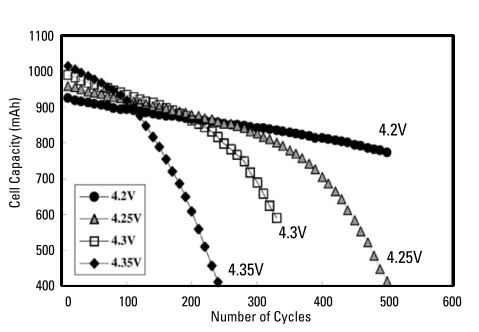
\includegraphics[width=0.6\textwidth]{bat_char/C_vs_Cycle_V.png}
    \caption{Relación Voltaje de carga la bateria vs Ciclos de vida de una celda de
Ion-Litio con un cátodo de $LiCoO_2$} \label{fig:C_vs_Cycle_V} \end{figure}
\FloatBarrier

A voltajes mayores el material del cátodo reacciona a mayor velocidad con el
electrolito perdiéndose material en la reacción resultando en una perdida de
capacidad de almacenamiento de energía. 

\subsubsection{Tenología Seleccionada}

Para un completo control del perfil de carga ariba descripto es que
seleccionamos circuito integrado \emph{bq24610} de la firma \emph{Texas
Instrument}.

El \emph{bq24610} es un circuito altamente integrado que implementa un cargador
de \acrfull{Ion-Li} o \acrfull{Li-Po} y capaz de operar de forma independiente o
stand-alone. Emplea un controllador de corriente y de tensión sincrónico
switching PWM de frecuencia constante y de alta resolución del tipo buck cuya
topología simplificada puede observarse en la figura \ref{fig:simp_sch_char}. 

\begin{figure}[h!]
    \centering
    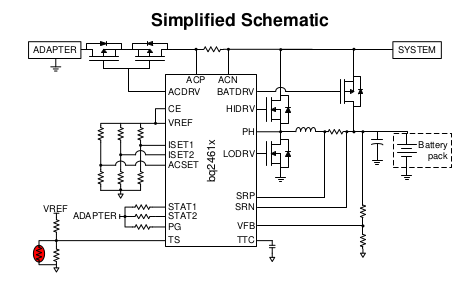
\includegraphics[width=0.5\textwidth]{bat_char/simp_sch_char.png}
    \caption{Esquema simplificado Cargador de Batería}
    \label{fig:simp_sch_char}
\end{figure}
\FloatBarrier

El mismo admite la conexión de hasta 6 celdas en serie con una tensión y
corriente máxima de entrada de hasta $28V$ y $10A$ respectivamente y una salída
de hasta $26V$ y $10A$ ajustandose adecuadamente a nuestros requerimientos y a
la topología de nuestro pack de baterías \emph{6S3P} descripta en \ref{batSel}.
El empaquedato del mismo es del tipo VQFN.

\subsection{Ecualización de celdas}

\noindent Como se comentó en secciones anteriores, cuando múltiples celdas se
encuentran conectadas en serie, el voltaje de una celda no siempre coincide con
la tensión equivalente del pack de baterías dividido por el número de celdas. 

\noindent La ecualización de celdas es una técnica en la cual se trata de
mantener los niveles de voltaje entre las celdas que conforman la cadena
conectada en serie de un pack de baterías de forma homogénea, es decir, que los
niveles de tensión entre celdas sea lo más uniforme posible, con el objetivo de
maximizar la eficiencia del pack de baterías.

\noindent El desbalance más típico generalmente se manifiesta en una variación
en el voltaje entre éstas, que puede ser corregido instantáneamente o
gradualmente conectando cargas externas en paralelo, a través de sus
correspondientes transistores, provocando una corriente de descarga adicional
que pueden ir desde miliamperes hasta varios Amperes, dependiendo del
dimensionamiento energético del pack de baterías. Sin embargo, este desbalance
en tensión es, por lo general, dado por desbalances químicos o distintas
dinámicas de descarga entre celdas, provocando que el objetivo del balanceo no
esté claramente definido provocando más perjuicios que beneficios al sistema
completo.  De hecho, la mayoría de las metodologías basadas en el desbalance de
voltaje, llevan a un pack de baterías más desbalanceado que sin ellos.

\noindent Por lo tanto es necesario conocer la naturaleza de los distintos tipos
de desbalances, los cuales son descriptos a continuación:

\subsubsection{Desbalance del estado de carga (SoC)}

\noindent El desbalanceo por estado de carga es causado por celdas que son
cargadas a distintos nivels de \acrshort{SOC}. Por ejemplo, si tenemos 3 celdas
cuya carga máxima es de 2200mAh ($\mathrm{Q_{max}}$), y descargar 100mAh una de
las celdas ($\mathrm{Q_1}$), la segunda por 100mAh y la tercera por 200mAh , la
primer y segunda celda van a estar a un \acrshort{SOC} de
$\mathrm{\frac{(Q_{max} - Q_1)}{Q_{max}} = 95.4\%}$. pero la tercer celda
estará, a cálculo hecho, en un 91\%. Por lo que podemos decir que la tercer
celda presenta un desbalance de un 4.4\%. 

Esto se traduce en distintos voltajes de circuito abierto, ya que se encuentran
directamente correlacionadas con el estado de carga de las mismas, sin embargo,
a pesar de esta diferencia constante de \acrshort{SOC}, la tensión entre celdas
varía con el crshort{SOC} debido a su variación con respecto a los distintos
niveles de estado de carga. En la Figura \ref{diff_imbalance} se muestra como
varía la diferencia de voltaje entre las celdas ante distintos niveles de
crshort{SOC} con un desbalance constante teniendo en cuenta la curva de la
figura \ref{OCV_SOC_equalization_figure}.

\begin{figure}[h!]
    \begin{subfigure}[t]{.5\textwidth}
	\begin{center}
	    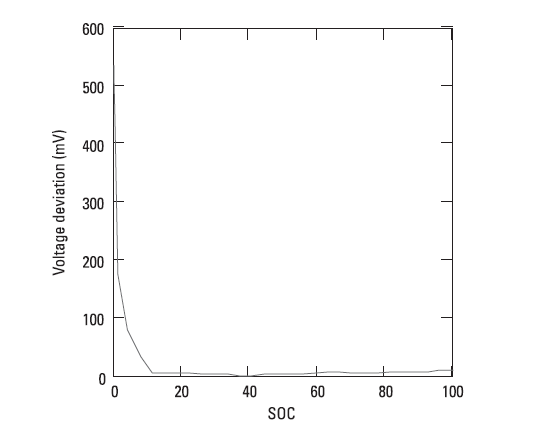
\includegraphics[width=0.9\textwidth]{diff_imbalance.png}
	    \caption{Diferencia de OCV a distintos estados de carga para un desbalance
	    de 1\% de SOC}
	    \label{diff_imbalance}
	\end{center}
    \end{subfigure}%
    ~
    \begin{subfigure}[t]{.5\textwidth}
	\begin{center}
	    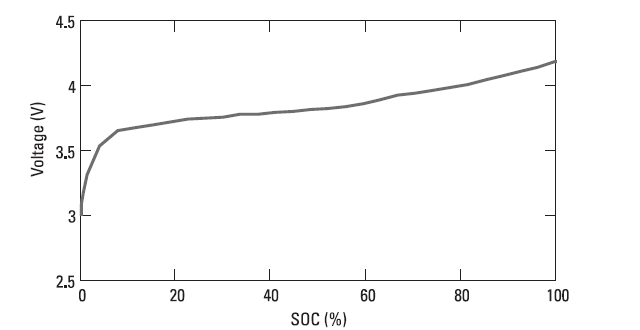
\includegraphics[width=0.9\textwidth]{SOC_vs_OCV_equalization.png}
	    \caption{OCV vs SOC}
	    \label{OCV_SOC_equalization_figure}
	\end{center}
    \end{subfigure}
    \caption{Variaciones del OCV segun SoC}
    \label{rep_OCV_SOC}
\end{figure}
\FloatBarrier

\noindent El voltaje sobre una carga puede ser aproximadamente, y rápidamente,
modelada por la siguiente ecuación:

\begin{equation}
    V = OCV(SoC) + I \times R(SoC)
    \label{v_load_bat}
\end{equation}

\noindent Debido a que la función $R(SOC)$ incrementa rápidamente a bajos
valores de SOC, la diferencia de voltajes entre celdas, con un desbalance de SOC
determinado, incrementa en un estado de carga muy bajo sugeriendo que existe un
incremento en la necesidad de realizar el proceso de balanceo cuando el pack de
baterías alcanza su descarga completa, sin embargo, si esta diferencia de SOC es
eliminada en etapas anteriores, las diferencias de tensión que ocurren cerca del
fin de descarga son eliminadas sin necesidad de altas corrientes de drenaje para
cada celda.

\subsubsection{Diferencias entre impedancias internas}

La diferencia entre impedancias internas en un bache de producción es de
aproximadamente un 15\% como se puede observar en la Figura \ref{zin_diff}.

\begin{figure}[h!]
    \begin{center}
	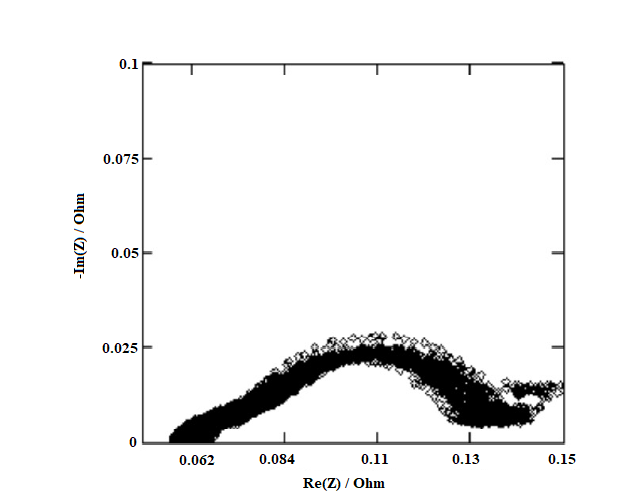
\includegraphics[width=0.7\textwidth]{zin_diff.png}
	\caption{Diferencias de espectrometrías entre 50 celdas. 
	El ensayo es realizado entre 1kHz a 10mHz}
	\label{zin_diff}
    \end{center}
\end{figure}
\FloatBarrier

Desbalances en la impedancia interna de la celda no causan diferencias en el
OCV, sin embargo, causará diferencias en el voltaje de la celda durante la
descarga, ya que la misma viene dada por la Ecuación \ref{v_load_bat}. Si la
batería se encuentra descargando, es decir, si la corriente es negativa el
voltaje que entrega a la carga será menor para una celda con mayor impedancia
interna. Por el otro lado, si la celda se encuentra cargando, el voltaje será
mayor para aquellas celdas con mayor resistencia interna.

A pesar de estas diferencias, no hay mecanismo de balanceo que permita solventar
el problema del desbalanceo de impedancia interna.

\subsubsection{Diferencias en la Capacidad de las celdas}

Por el otro lado, puede suceder que la capacidad química de las celdas
($\mathrm{Q_{MAX}}$) pueden ser diferentes en un principio, esto provoca que, a
pesar de que cada celda sea descargada por la misma cantidad de corriente, el
estado de carga será diferente. Por ejemplo, si las 3 celdas que nombramos
anteriores son descargadas por 100mAh, pero la 3er celda tiene una capacidad
distinta al resto (por ejemplo, 2000mAh en vez de 2200mAh), los estados de carga
resultantes serán de 95.4\% y 95\%.

Nuevamente esto provocará una diferencia en los OCVs de las celdas. Como puede
observarse, 200mAh de diferencia en $\mathrm{Q_{MAX}}$ causa solamente una
diferencia de un 0.4\% en el SOC, causando menor diferencia de voltaje que un
desbalance en el estado de carga.

Teniendo esto en cuenta las baterías no podrán estar balanceadas durante todo el
ciclo de descarga o de carga ya que al quitar la misma cantidad de carga el
estado de carga de las mismas será distinto. Un ejemplo algo más gráfico de esto
es con 2 vasos de agua, uno con el doble de capacidad del otro pero llenos hasta
la misma altura. Si se remueve la misma cantidad de agua de ambos el de mayor
capacidad se habrá descargado la mitad que el de menor capacidad.

En la práctica lo más común es lo que se llama \emph{top balancing}, que implica
balancear en el período de carga todas las celdas del pack al 100\%. El mismo
consiste descargar las celdas de menor capacidad permitiendo a las celdas de
mayor capacidad un margen para seguir cargando sin sobrecargar las primeras,
evitando lo que generaría una drástica disminución de la vida útil del pack.
Esta opción es mucho más atractiva que su contra parte denominada \emph{bottom
balancing} ya que esta balancea todas las baterías a su estado de carga en 0\%,
lo cual no acarrea ninguna ventaja ya que el pack de baterías va a seguir
entregando a la carga la misma cantidad de energía, esto es, cuando la batería
de menor capacidad se descargue como pasaría si no se realizara el balanceo
inferior.

La descarga de las celdas se puede llevar a cabo disipando su energía en
resistores o transfiriendo la carga a las celdas más descargadas, siendo estos
métodos clasificados como balanceo pasivo o balanceo activo respectivamente. Los
métodos pasivos son mucho más sencillos y económicos y en la mayoría de los
casos no es justificado el uso del método activo ya que los circuitos que llevan
a cabo la transferencia de energía poseen perdidas por lo que no ofrecen
ventajas reales en aplicaciones de baja potencia.

Por el otro lado, puede suceder que la capacidad química de las celdas
($\mathrm{Q_{MAX}}$) pueden ser diferentes en un principio, esto provoca que, a
pesar de que cada celda sea descargada por la misma cantidad de corriente, el
estado de carga será diferente. Por ejemplo, si las 3 celdas que nombramos
anteriores son descargadas por 100mAh, pero la 3er celda tiene una capacidad
distinta al resto (por ejemplo, 2000mAh en vez de 2200mAh), los estados de carga
resultantes serán de 95.4\% y 95\%.

Nuevamente esto provocará una diferencia en los OCVs de las celdas.  Como puede
observarse, 200mAh de diferencia en $\mathrm{Q_{MAX}}$ causa solamente una
diferencia de un 0.4\% en el SoC, causando menor diferencia de voltaje que un
desbalance en el estado de carga.

Teniendo esto en cuenta las baterías no podrán estar balanceadas durante todo el
ciclo de descarga o de carga ya que al quitar la misma cantidad de carga el SoC
de las mismas será distinto. Un ejemplo algo más gráfico de esto es con 2 vasos
de agua, uno con el doble de capacidad del otro pero llenos hasta la misma
altura. Si se remueve la misma cantidad de agua de ambos el de mayor capacidad
se habrá descargado la mitad que el de menor capacidad.

En la práctica lo más común es lo que se llama \emph{top balancing}, que implica
balancear en el período de carga en la que el pack se considera cargado a un
100\% o durante el periodo de Tension constante o CV (del ingles \emph{Constant
Voltage}). El mismo consiste descargar las celdas de menor capacidad permitiendo
a las celdas de mayor capacidad un margen para seguir cargando sin sobrecargar
las primeras, evitando lo que generaría una drástica disminución de la vida útil
del pack. Esta opción es mucho más atractiva que su contra parte denominada
\emph{bottom balancing} ya que esta balancea todas las baterías a su estado de
carga cercano al 0\%, lo cual no acarrea ninguna ventaja ya que el pack de
baterías va a seguir entregando a la carga la misma cantidad de energía, esto
es, cuando la batería de menor capacidad se descargue como pasaría si no se
realizara el balanceo inferior.

La descarga de las celdas se puede llevar a cabo disipando su energía en
resistores o transfiriendo la carga a las celdas más descargadas, siendo estos
métodos clasificados como balanceo pasivo o balanceo activo respectivamente. Los
métodos pasivos son mucho más sencillos y económicos y en la mayoría de los
casos no es justificado el uso del método activo ya que los circuitos que llevan
a cabo la transferencia de energía poseen perdidas por lo que no ofrecen
ventajas reales en aplicaciones de baja potencia.

Por último hay que considerar que corriente es necesaria para balancear el pack,
a mayor capacidad de corriente las corrientes de auto descarga y cambios en la
capacidad por envejecimiento van generando pequeños desbalances, pero los mismos
son acotados, las corrientes de auto descarga generan desbalances menores al
0.1\% por ciclo. 

\begin{figure}[h!]
    \begin{center}
	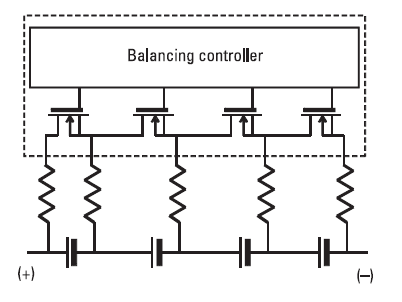
\includegraphics[width=0.5\textwidth]{passive_equalizator.png}
	\caption{Esquemático de conexión de un balanceador pasivo.}
	\label{passive_equalizator}
    \end{center}
\end{figure}
\FloatBarrier

%Para la implementación del balanceador analizó LTC6803-2.

El integrado BQ76PL536 de texas instrument es un Monitor de batería con
protecciones para sobre  y sub tensión y sobrecalentamiento asi como también
posee varias funcionalidades entre las cuales se destacan la posibilidad de
escalar el número de celdas en serie gracias a su interfaz D2D VBUS
(\emph{device to device vertical BUS}) permitiendo la conexión en serie de
varios BQ76PL536 permitiendo controlar hasta 6 celdas por integrado hasta un
total de 192 celdas.
%Anteriormente se nombró la importancia de la protección de las celdas, ya que
%el voltaje de ruptura del electrolito es cercano a la tensión de carga máxima
%de una celda (entre 4.1V a 4.3V por celda). Por lo tanto, se debe realizar un
%control y monitoreo riguroso para que las celdas de un pack experimente un
%sobrevoltaje durante el proceso de carga. Esto, conlleva a que, en un pack de
%baterías, cada celda sea monitoreada y controlada por separado, ya que
%controlar la tensión del pack de baterías no es suficiente, debido a que, a
%pesar de que los valores pueden encontrarse dentro de un umbral correcto, una
%de las celdas que componen el sistema puede estar experimentando un daño
%permanente por sobrevoltaje debido al desbalance que pueden encontrarse entre
%celdas

%El balanceo de celdas es necesario para aquellas aplicaciones donde tienen
%grandes transitorios de energía, especialmente aquellas aplicaciones donde
%ocurre frecuentemente, como por ejemplo, los frenos regenerativos en los EVs y
%HEVs. El freno regenerativo puede causar grandes flujos de corriente provocando
%un incremento instantáneo en la tensión de cada celda, alcanzando la tensión de
%ruptura del electrolito.

%Las desviaciones en las celdas generalmente ocurren debido a dos fenómenos:
%cambios en la impedancia interna o en la reducción de capacidad debido al
%envejecimiento de las mismas. En ambos casos, si una celda experimenta una
%desviación en su comportamiento, esta celda es un posible candidato a un
%sobrevoltaje durante los eventos que ocurren los transitorios de potencia. Las
%celdas con capacidad reducida o alta impedancia interna tienden a tener altas
%variaciones de tensión durante los procesos de carga y descarga.
%
%Por último, en aplicaciones donde es deseable obtener la mayor capacidad usable
%de un pack de baterías, puede ocurrir que durante el proceso de carga, una
%celda desbalanceada alcance el voltaje de fin de carga y provoca que el proceso
%de carga termine prematuramente. Entonces, además de proteger el pack de
%baterías, el proceso de carga permite aprovechar la capacidad completa del pack
%a pesar de los desbalanceos intrínsecos de cada celda.
%
%Tradicionalmente, los desbalances entre celdas en baterías de plomo son
%solucionados por una sobrecarga controlada. Este tipo de baterías pueden ser
%llevadas a condiciones de sobrecarga sin ser dañadas permanentemente, ya que el
%exceso de energía es liberado a través de la gasificación de las sustancias
%químicas que contienen. Éste método, es el método natural para el balanceo de
%celdas de plomo-ácido conectadas e nserie. Otras composiciones químicas, tales
%como las de Niquel-metal, exhiben un mecanismo similar.
%
%Debido a que las baterías de Litio no pueden ser sobrecargadas, no existe un
%mecanismo natural para el balanceo de celdas. Por lo tanto, se deben emplear
%métodos diferentes para balancearlas. Los métodos de balanceo se pueden separar
%en dos grandes grupos: Métodos activos y pasivos.
%
%A continuación, se describen los métodos más comunes para realizar el balanceo
%de celdas.

%\subsubsection{Balanceo de Celdas en el Fin de carga}

%Este método es empleado cuando el pack de baterías cuando es cargada
%completamente y es, generalmente, implementada en aquellas aplicaciones en las
%cuales el pack de baterías es completamente cargado en cada ciclo de su uso.
%Como pueden ser en fuentes de baterías ininterrumpidas (UPS, del inglés
%\emph{Uninterruptible Power Supply}) o vehículos eléctricos hasta celulares. 

\subsection{Plan de Trabajo}

Se plantea el siguiente plan de trabajo con el tiempo estimado para la
finalización del proyecto:

\begin{table}[h!]
    \begin{tabular}{|l|c|}
	\hline
	\multicolumn{1}{|c|}{Tarea}                                                                                                                                                                              & Duración                           \\ \hline
	\begin{tabular}[c]{@{}l@{}}Estudio, análisis y comparación del estado del arte de la tecnología. \\Estudio de los requerimientos de hardware.\end{tabular}                         & 2 Semanas                          \\ \hline
	    \begin{tabular}[c]{@{}l@{}}Modelado de baterías de Li-Ion en MatLab. \\Simulación de los distintos algoritmos y los circuitos de protección. \\ Estudio y comparación. Validación y elección de los más adecuados.\end{tabular} & 4 Semanas                          \\ \hline
		\begin{tabular}[c]{@{}l@{}}Desarrollo e implementación del hardware del \acrshort{BMS}. *\end{tabular}                                                      & 6 Semanas                          \\ \hline
		    \begin{tabular}[c]{@{}l@{}}Desarrollo del Firmware del \acrshort{BMS} con los algoritmos seleccionados.\\  Implementación y depuración sobre el hardware.\end{tabular}                                                    & 4 semanas                          \\ \hline
			Montaje del banco de pruebas para ensayar las protecciones y los algoritmos correspondientes. *                                                                                                                       & 3 Semanas                          \\ \hline
			Análisis de resultados, obtención de conclusiones y desarrollo del informe final.                                                                                                                                                       & 3 Semanas                          \\ \hline
			\textbf{Total}                                                                                                                                                                                                  &\textbf{24 Semanas} \\ \hline
    \end{tabular}
\end{table}

\subsection{Extensión a futuros proyectos}

El desarrollo del hardware y los algoritmos, tanto de ecualización como de
estado de carga sirven como una buena base para futuros proyectos vinculados a
la temática de energías renovables y \acrshort{VE}s.

Como posible extensión se plantea el desarrollo de algoritmos novedosos para la
estimación del Estado de Salud, su posible aplicación a sistemas de alta
potencia e inclusive realizar estudios sobre nuevas tecnologías relacionadas a
la composición química de las celdas.

\newpage

\section{Desarrollo}\label{desarrollo}
(Sección en desarrollo)
%\subsection{Implementación Circuito Cargador}

% La carga del pack de batería no es un proceso trivial y la extensión de la
% vida util del mismo depende profundamente de poder controlar el mismo con
% detalle. 

% El control completo de la operación del pack de batPoder controlar Extender la
% vida util del pack de baterías no es un tema trivial como ya hemos expuesto
% anteriormente. El balanceo de carga es

\section{Ensayos}\label{ensayos}
(Sección en desarrollo)
%TODO: Ensayos
\newpage

\section{Conclusiones}\label{conclusiones}
(Sección en desarrollo)
%TODO: Conclusiones
\printbibliography
\newpage
% Print table of acronyms
\addcontentsline{toc}{section}{Tabla de Abreviaturas}
\glsaddall
\printnoidxglossary[type=\acronymtype,title={Abreviaturas}]

\end{document}
\documentclass[10pt,a4paper]{article}
